% !TeX spellcheck = en_US
\documentclass[
  fontsize=12pt,
  bibliography=totoc,
  numbers=noenddot,
  listof=totoc,
  %toc=totoc,
  appendixprefix,
  oneside,  %  twoside=semi,
  paper=a4,
  % test
  headings=small,
%  parskip=full
]{scrbook} % scrbook  memoir
\setcounter{tocdepth}{2}                                 % levels which are displayed in the table of contents
%
% Packages
% -----------------------------------
\usepackage[
  paper=a4paper,
  left=12.5mm,
  right=25mm,
  top=25mm,
  bottom=25mm,
%  showframe,
  bindingoffset=10mm]{geometry}                            % page and binding margins can be adjust here

\usepackage{inputenc}                                 % mutated vowel (Umlaute) in the text
\usepackage[british]{babel}                                 % orthography
\usepackage{csquotes}                                       % Context sensitive quotation
%\usepackage[utf8]{fontenc}                                 % for better encoding --
\usepackage{lmodern}                                        % font family
\usepackage{microtype}                                      % for micro typography (for a better typeface)
\usepackage{graphicx}                                       % for including graphs (pdf,png - but do avoid jpg)
\graphicspath{{./img/}{../../output/figures}}                                     % path to the pictures
\usepackage{grffile}
\usepackage{xcolor}
\definecolor{White}{rgb}{1,1,1}
\definecolor{cp}{gray}{0.92}
\definecolor{cm}{gray}{0.96}
\definecolor{LightCyan}{rgb}{0.88,1,1}
\usepackage[hyphens]{url}                                   %  formatting URL (e.g. in the literature)

\usepackage{tabularx}                                       % for a better configuration of tables
\usepackage{longtable}
\usepackage{multicol}
\usepackage{multirow}
\usepackage{booktabs}
\usepackage{afterpage}

\usepackage[flushleft]{threeparttable}
\usepackage[active]{srcltx}

\usepackage{siunitx}
\sisetup{group-separator=\, ,
        output-exponent-marker = \text{e},
        exponent-product={},
        retain-explicit-plus,
        input-open-uncertainty  = ,
        input-close-uncertainty = ,
        table-align-text-pre    = false,
        group-minimum-digits={4},
%        round-mode=places,
        table-space-text-post = \sym{***},
        table-space-text-pre    = (,
        table-space-text-post   = ),
        table-align-text-post=false,
} % centering in tables} % centering in tables

%\usepackage{listings}                                       % for computer code output
% \usepackage{inconsolata}

\usepackage{mdwlist}                                        % lists

\usepackage{setspace}                                       % setting of the lines (rows)
%\newtheorem{mydef}{Merksatz}                               % if examples or mnemotechnic verses are used with continuous numeration
%\newtheorem{bsp}{Beispiel}

%\usepackage{todonotes}                                     % for the creation of ToDos
\usepackage{lscape}                                         % for the rotation of pages

%\usepackage{tikz}
%\def\checkmark{\tikz\fill[scale=0.4](0,.35) -- (.25,0) -- (1,.7) -- (.25,.15) -- cycle;} 

% -------------------------------------------------------------------------------------------------
% math packages ----
% -------------------------------------------------------------------------------------------------
%\usepackage{amsmath}                                        % for the writting of mathematical formula
\usepackage{amsmath,amssymb}
\DeclareMathOperator{\E}{\mathbb{E}}
\DeclareMathOperator{\sign}{sign}
\providecommand{\abs}[1]{\lvert#1\rvert}
\usepackage{unicode-math}
%\usepackage{bm}
\usepackage{calc}
%\usepackage{footnote}                                      % footnotes
\usepackage{tablefootnote}                                  % footnotes in tables

% test test
\usepackage{caption} % 'format=plain' avoids hanging indentation
\captionsetup{
  font=normalsize,
  labelsep=quad,
  labelfont={sf,bf},
  justification=justified, %justified, raggedright
  singlelinecheck=false
  }
\usepackage[
    font=footnotesize,
    justification=centering,
    subrefformat=parens,
    labelformat=parens]{subcaption}

\captionsetup[sub]{labelfont=bf, labelformat=brace, subrefformat=simple}
% fnote command to use as notes for figures
\newcommand\fnote[1]{
    \captionsetup{
        font=footnotesize, 
        justification=justified,
        singlelinecheck=false}\vspace*{-.3\baselineskip}\caption*{#1}
}




%% end subcaption

\usepackage[
    linktocpage=true,
    colorlinks]{hyperref}                 % For hperlinks in PDF-documents

\hypersetup{%
    colorlinks=false,% false: hyperlinks will be black
    linkcolor=blue,
    linkbordercolor=blue,% hyperlink of cref borders 
    urlcolor=blue,
    urlbordercolor=white,
    citecolor=blue,% if colorlinks true
    citebordercolor=blue,% hyperlink of citation
    pdfborderstyle={/S/U/W 1}% border style will be underline of width x pt, 
    }
\hypersetup{%
    pdftitle={The health-wealth nexus over the life cycle},
    pdfsubject={Master Thesis in Economics at FU-Berlin},
    pdfauthor={Marcelo Rainho Avila},
    pdfproducer={TeXstudio + xelatex},
    pdfcreator={Marcelo Rainho Avila}
}

\usepackage[noabbrev,capitalise,nameinlink]{cleveref}
%\crefname{chapter}{Section}{Sections}

\usepackage{bookmark} %%https://tex.stackexchange.com/questions/30330/how-can-i-avoid-compiling-twice


\usepackage{enumitem}

% hack 
\usepackage{scrhack}
\usepackage{adjustbox}
\usepackage{float} % here for H placement parameter
\usepackage{appendix}
\usepackage{colortbl}

\usepackage{pdflscape}

%\pdfminorversion=6

% bibliography --
\usepackage[
    backend=biber,
    sortcites=false,
    style=authoryear-icomp, %authoryear-icomp
    doi=true,
    isbn=false,
    url=false,
    eprint=false, % https://tex.stackexchange.com/questions/23117/
    %backref=true,
    giveninits=true,
    uniquename=init,
    dashed=false,
    bibencoding=utf8,
    hyperref,
    maxcitenames=2]{biblatex}
    %authoryear, %bibstyle=draft, %sorting=nyt,
\setlength\bibitemsep{1.5\itemsep}

\addbibresource{./literature/sources.bib}                   % including literature sources
\DeclareLabeldate{\field{date}\field{eventdate}\field{origdate}\field{year}\literal{nodate}}
\renewcommand*{\nameyeardelim}{\addcomma\space}

\DefineBibliographyStrings{english}{%
    backrefpage = {page},% originally "cited on page"
    backrefpages = {pages},% originally "cited on pages"
}

\AtEveryBibitem{%
    \ifboolexpr 
    { % test 
        test {\ifentrytype{online}}
        or 
        test {\ifentrytype{software}}
    }
    { % true , do nothing
    }
    { % false
        \clearfield{month}%
        \clearfield{day}%
    } 
}


\DeclareCiteCommand{\citeauthor} % https://tex.stackexchange.com/questions/75902
{\boolfalse{citetracker}%
    \boolfalse{pagetracker}%
    \usebibmacro{prenote}}
{\ifciteindex
    {\indexnames{labelname}}
    {}%
    \printtext[bibhyperref]{\printnames{labelname}}}
{\multicitedelim}
{\usebibmacro{postnote}}

% https://tex.stackexchange.com/questions/1687/hyperlink-name-with-biblatex-authoryear
\DeclareFieldFormat{citehyperref}{%
    \DeclareFieldAlias{bibhyperref}{noformat}% Avoid nested links
    \bibhyperref{#1}}

\DeclareFieldFormat{textcitehyperref}{%
    \DeclareFieldAlias{bibhyperref}{noformat}% Avoid nested links
    \bibhyperref{%
        #1%
        \ifbool{cbx:parens}
        {\bibcloseparen\global\boolfalse{cbx:parens}}
        {}}}

\savebibmacro{cite}
\savebibmacro{textcite}

\renewbibmacro*{cite}{%
    \printtext[citehyperref]{%
        \restorebibmacro{cite}%
        \usebibmacro{cite}}}

\renewbibmacro*{textcite}{%
    \ifboolexpr{
        ( not test {\iffieldundef{prenote}} and
        test {\ifnumequal{\value{citecount}}{1}} )
        or
        ( not test {\iffieldundef{postnote}} and
        test {\ifnumequal{\value{citecount}}{\value{citetotal}}} )
    }
    {\DeclareFieldAlias{textcitehyperref}{noformat}}
    {}%
    \printtext[textcitehyperref]{%
        \restorebibmacro{textcite}%
        \usebibmacro{textcite}}}


% inline code environment
\let\code=\texttt

% for esttab estout table output
\def\sym#1{\ifmmode^{#1}\else\(^{#1}\)\fi}

% for expliciting topic (unnumberd subsection)
%\newcommand{\topic}[1]{\vspace{.5em}\noindent\textbf{#1}\qquad}
\newcommand{\topic}{\subsubsection}

% short for \textsubscript
\newcommand{\tsub}[1]{\textsubscript{#1}}
\newcommand{\tsup}[1]{\textsuperscript{#1}}


% hook 
\ExplSyntaxOn % providing \expandableinput
\cs_new:Npn \expandableinput #1
{ \use:c { @@input } { \file_full_name:n {#1} } }
\ExplSyntaxOff

\makeatletter

\renewcommand\thesubfigure{\alph{subfigure}}
\renewcommand\p@subfigure{\thefigure\,}

% https://tex.stackexchange.com/a/122465/145182 Subsubsection: remove the newline (like paragraph)
\renewcommand\subsubsection{\@startsection{subsubsection}{3}{\z@}%
    {-3.25ex\@plus -1ex \@minus -.2ex}%
    {-1.5ex \@plus -.2ex}% Formerly 1.5ex \@plus .2ex
    {\normalfont\normalsize\bfseries}}

\makeatother


% Document
% -----------------------------------
\begin{document}


\frontmatter
    % Title page shall not include header or foooter lines
\thispagestyle{empty}

% All elements shall be centered
\begin{center}


\Large\textsc{Chair of Public Finance and Social Policy}\\%
of the\\%
\Large\textsc{Free University Berlin}%

\vspace*{1cm}
\includegraphics[width=.25\textwidth]{fu_logo}

\vspace*{1cm}
\Large{Master Thesis}\\ 
\vspace{1.5cm}

\centering \huge The health--wealth nexus\\over the life cycle

\vspace{3cm}

{\Large Marcelo Rainho Avila}\\[15mm]

\end{center}

\vfill

% Superverisor, contact data and submission date
\begin{normalsize}
    \begin{center}
        \begin{tabular}{lr}
            Supervisor:              & Prof. Dr. Carsten Schröder\\[24pt]
            Address:                 & Seestraße 100, 13353, Berlin\\[3pt]
            Email:                   & m.avila@fu-berlin.de\\[3pt]
            Submission:              & 07.02.2024  \\[3pt]
            Matriculation-Nr.:       & 4679876\\[3pt]
        \end{tabular}
    \end{center}
\end{normalsize}


\clearpage{\pagestyle{empty}\cleardoublepage}                                   % title
%    \thispagestyle{empty}
\vspace*{1cm}
\phantomsection
\addcontentsline{toc}{chapter}{Abstract}
\begin{center}
\textbf{Abstract}
\end{center}
\vspace*{1.5cm}
\noindent 

It is a long-established fact that a reader will be distracted by the readable content of a page when looking at its layout. The point of using that is that it has a more-or-less normal distribution of letters, as opposed to using 'Content here, content here', making it look like readable English. Many desktop publishing packages and web page editors now use that as their default model text, and a search for 'lorem ipsum' will uncover many websites still in their infancy. Various versions have evolved over the years, sometimes by accident, sometimes on purpose (injected humor and the like).                          % abstract
     \tableofcontents                                       % table of contents
    \clearpage
\begingroup
    \let\cleardoublepage\relax
    \listoffigures                                          % list of figures
\endgroup
\begingroup
    \let\clearpage\relax
    \let\cleardoublepage\relax
       \listoftables                                       % list of tables
\endgroup

% -----------------------------------

\mainmatter                                                 % the respective chapters

\onehalfspacing                      % line spacing which is set to 1.5 from this point on


\nocite{
    rios-avila.etal2023csdid,
    rios-avila.etal2024csdid2,
    statacorp.2023stata,
    correia2023reghdfe}

	% !TeX spellcheck = en_US
% !TeX root = ../ma_mravila.tex

% -------------------------------------------------------------------------------------------------
% Intro
% -------------------------------------------------------------------------------------------------

%\input{./chapter/01_introduction.tex}

\chapter{Introduction}

\vspace{60pt}

``The first wealth is health.'' \quad In 1860, the philosopher Ralph Waldo Emerson posited that good health is
a precondition to flourishment and living a fulfilling life.  Since then, researchers have shown that people with higher socioeconomic status live healthier and longer lives (see \cite{deaton2003health,case.deaton2005broken,chetty.etal2016association}). %
%

While these results replicate across diverse societies and periods, the exact mechanisms are still open to
discussion. To what extent wealth causes health or, conversely, health causes wealth is not trivial to disentangle
given the nature of these variables. In a meta-analysis, \citeauthor{kröger.etal2015what} find evidence in both
directions \autocite{kröger.etal2015what}. It is not difficult to think of possible mechanisms. People with higher
socioeconomic status might, for example, have access to better health care or live in areas with more opportunities for following healthier life styles. On the other hand, good health might be a prerequisite for achieving
financial success, as it enables individuals to participate fully in the workforce and pursue educational and career
opportunities. Despite these broad associations, the specific pathways through which health influences wealth
accumulation remain complex. This study aims to contribute to this discussion by focusing specifically on the
pathway from health to wealth accumulation, quantifying how adverse health outcomes impact individuals' wealth
trajectories over time. Further, by analyzing mental and physical health shocks separately, the effects from
both domains can be compared to one another. 


\cref{fig:wealthbyageovertreated} serves to illustrate the difference in wealth trajectory over the life cycle
between two groups: those who experience a significant adverse health outcome over the life cycle, and those who do
not. Although the starting values, on average, are on the same level earlier in life, one group manages to build up
considerably more wealth than the other. By age 60, the group with a more stable health
trajectory accumulates 35\% (gross) and 40\% (net) more wealth than their counterpart.
This work aims to explore if, and to what extent, an adverse health outcome, whether in the mental or physical
domain, helps explain the observed difference in this figure.


On these accounts, this analysis employs a Difference-in-Differences (DiD) method with multiple time periods and
variation in treatment timing to estimate the causal effect of an adverse health outcome on the wealth trajectory
of adults in Germany. The unbalanced panel data employed in this work are provided by the German Socio-Economic
Panel (SOEP). The final sample encompasses people aged between 18 and 75 and provides, among other variables, health and wealth 
information since 2002. It includes over 16 thousand individuals and more than 80 thousand observations.


This work is structured as follows: \cref{sec:overview_did} presents an overview of the DiD framework proposed by
\textcite{cs2021did_mtp}. \cref{chap:data} describes the data and focal variables used in this study.
\cref{sec:meas_health} focuses on the measurement of health and, as a secondary analysis, evaluates some of the
criticisms raised in the literature about uncorrelated health summary scores. Further, the alternative method for
computing the summary scores used in this analysis is introduced. \cref{chap:empir_metho_res} covers the empirical
approach and focuses on the results obtained in the main analysis. Also in this chapter, secondary analyses are
presented. They explore wealth accumulation links and evaluate effect heterogeneity by education attainment and age
groups, as well as a section on robustness checks. \cref{ch:discus} presents a discussion on the obtained results,
including a section on threat to internal validity and another on extensions to the current study. Finally,
\cref{ch:conclus} summarizes the findings in this study.




\begin{figure}[t]
    \centering
    \begin{subfigure}{.45\textwidth}
        \centering
        \caption*{\small Gross Wealth}
        \includegraphics[width=.95\linewidth]{../../output/figures/csdid2/h_descr/wealth_by_age_over_treated_gw.pdf}
    \end{subfigure}
    \begin{subfigure}{.45\textwidth}
        \centering
        \caption*{\small Net Wealth}
        \includegraphics[width=.95\linewidth]{../../output/figures/csdid2/h_descr/wealth_by_age_over_treated_nw.pdf}
    \end{subfigure}
    \caption{Wealth trajectory by treatment status}
    \fnote{ \footnotesize Notes: Figure shows two-year moving average with whiskers depicting the 99\% confidence intervals. 
        Untreated refer to those that did not experience a adverse health outcome up to a given age,
        while post-treated refer to those treated from the respective certain age onward. For brevity, only the treatment relative to mental health domain is shown. Sample composition changes over life cycle, as the longest time span for a single individual is 19 years. 
        Data source: SOEPv37}
    \label{fig:wealthbyageovertreated}
\end{figure}





% -------------------------------------------------------------------------------------------------
% chapter diff in diff overview ----
% -------------------------------------------------------------------------------------------------
\chapter{Overview of DiD with Staggered Treatment from Callaway and Sant'Anna (2021)}
\label{sec:overview_did}

In recent years, numerous authors have advanced the Difference-in-Differences
design literature by addressing the ``forbidden comparisons'' issue, term coined and explained in
\textcite[14]{borusyak.etal2024revisiting}. In short, it arises when comparing later treated to early
treated units in a staggered DiD setting in the presence of effect heterogeneity. One of these approaches was proposed by
\textcite{cs2021did_mtp}, which is not only robust to this issue but offers other compelling
features, as discussed below. For an overview on the recent methods refer to the extensive survey from
\textcite{dechaisemartin.dhaultfoeuille2022twoway}.

In the following section I present an overview of the estimator as proposed from
\textcite{cs2021did_mtp}. I include only the sections that are relevant to this analysis,
while variations and other considerations are left out. For consistency, I borrow the terminology from the authors
for this analysis. In particular, I use terms such as ``comparison'' units instead of commonly used
``control'' units. I also use the term ``group'' which can be exchanged for ``cohort''.


\section{Building Blocks}

In short, the proposed estimator can be divided into two steps. First, compute the differences of valid
comparison groups in several simple, balanced 2-periods by 2-groups DiD designs. Then, aggregate
these estimations in a meaningful way. Adapting the notation of Eq. 2.8 from
\parencite{cs2021did_mtp}, the groups in the first step can be defined by their respective treatment
period $g$ and the measurement time $t$. So each group-time Average Treatment Effects on the Treated, 
hereafter $ATT(g,t)$ is defined as%
%
\begin{equation} 
    ATT(g,t) = \E \big[ Y_{t} - Y_{g-1} | G_{g}=1 \big]  -  \E \big[ Y_{t} - Y_{g-1} |
    C=1 \big], 
    \label{eq:attgt}
\end{equation}
%
where the conditional terms $G_g=1$ identifies the group first treated at period $g$ and $C=1$
determines the comparison units.%
\footnote{Note that the authors introduce two approaches that differs in terms of comparison units.
    One uses never-treated only, while the other uses also not-yet-treated units as comparison. I focus
    here on the never-treated specification, which is used in the main analysis, due to the risk of
    anticipation effects biasing the results.} %
%
This is the \textit{group-time average treatment effect}, as defined by the authors
\parencite*[Section 2.2]{cs2021did_mtp}. Since each one of these groups is by construction, a
canonical DiD design, they are valid comparisons and do not suffer from the ``negative weights''
issue.

In the second step, the \textcite{cs2021did_mtp} propose different ways of aggregating all $ATT(g,t)$'s.
In the main analysis, I follow the event study aggregation. For that, a relative-time 
variable $e = t-g$ is defined, which identifies time elapsed since treatment adoption. The target 
parameter is
%%
%
\begin{equation}
    \theta_\text{es}(e) = \sum_{g \in \mathcal{G}} \mathbb{1}\big[ g + e \leq \mathcal{T} \big] P(G=g|G+e \leq \mathcal{T}) ATT(g,g+e), 
    \label{eq:theta_es}
\end{equation}
%
where $\mathcal{T}$ is the last period in the analysis. The two new terms in the above summation are, first,
the indicator function that restricts the group-time average treatment effects. And second, the term $P(.)$ are
the group weights, so that the summation produces an average - weighted by group size - of all $ATT(g,t)$'s
included in the aggregation.


Note that this aggregation may suffer from compositional changes, which will have important implications, as
explained thoroughly in \textcite[see Equation 3.5]{cs2021did_mtp}. In short, the authors show that there are
two approaches to handling it: either restricting the analysis to a balanced sample or, alternatively, relying
on the additional assumption that the effects are equal across groups. That is, $ATT(g,g+e)$ does not vary with
$g$ for any $e \geq 0$. In the main analysis, I make the equal-effects assumption, but robustness checks with
sample restrictions do not change the results considerably.

\section{Summary Measures}

After computing the $ATT(g,t)$'s, there are a few choices of overall aggregation to obtain a single
parameter estimating the effect being assigned to treatment. As proposed by \textcite[Section
3.2]{cs2021did_mtp}, an intuitive one would be

\begin{equation}
    \overbar{\theta}_\text{simple} = \frac{1}{k} \sum_{g \in \mathcal{G}}^{} 
    \sum_{t=2}^{\mathcal{T}} \mathbb{1}\big[ t \geq g \big] ATT(g,t) P(G=g|G \leq \mathcal{T}), 
    \label{eq:didsimp}
\end{equation}
%
where $k=\sum_{g \in \mathcal{G}} \sum_{t=2}^{\mathcal{T}} \mathbb{1}\big[ t \geq g \big]
ATT(g,t) P(G=g|G \leq \mathcal{T})$. Another aggregation target proposed is relevant for the
event-study structure applied here. We can obtain an overall treatment effect by averaging
$\theta_{es}(e)$ over all event times, as in%
%
\begin{equation}
    \overbar{\theta}_\text{es} = \frac{1}{\mathcal{T-1}} \sum_{e=0}^{\mathcal{T}-2}{\theta_{es}(e)}.
    \label{eq:didpostpast}
\end{equation}

While the authors propose other summary measures, these are the relevant ones examined in this
analysis and presented in \cref{sec:Results}. %todo: cross ref main results

\section{Doubly-Robustness}

\citeauthor{cs2021did_mtp} propose three approaches to achieve an estimator capable of conducting
inference on the group-time average treatment effects \autocite[Sec. 4]{cs2021did_mtp}. In short, the Outcome
Regression, a generalization of the approach in \textcite{heckman.etal1997matching}, requires the evolution of
the response variable of the comparison group to be modeled correctly to ensure conditional parallel trends.
The second approach, building on inverse probability weighting (IPW) proposed by
\textcite{abadie2005semiparametric}, requires correct estimation of the conditional probability of being in
group $g$.


The doubly-robust method, extending the simpler DiD estimator from
\textcite{santanna.zhao2020doubly} to allow for multiple \textit{group-times}, is particularly appealing
because it can be seen as a combination of both approaches, modeling the response variable evolution
as well as the propensity score, but it only requires one to be correctly specified. Thus the 
term ``doubly robust''. 


For a more detailed view on the proposed estimator, see \cref{app:drdeep}. A closer look at
\cref{eq:wgtreatcomp} shows that the treated group are not re-weighted (or all receive unit
weights). Further, the subscripts in $\widehat{ATT}_{d r}(g, t)$, in \cref{eq:attdr}, hints that
this procedure is conducted for each one of the 2-by-2 group-time $ATT$, which entails important
implications: the same comparison units, those that are never treated in this case, are used for all
group-time estimations but receive different weights in each \textit{step}.


The implication is that it is not trivial to extract and store the weights from the IPW procedure.%
\footnote{The main author of the \code{csdid} package for Stata \parencite{rios-avila.etal2023csdid}
    confirms this in the Statalist forum \parencite{rios-avila2023SLWeights}. One could extract the
    weights from each treatment time cohort, and use them for further checks. In a setting with
    more than a few cohorts, however, this quickly becomes infeasible.} This means that while
this procedure doubly robust and automatically ``balances'' treatment and comparison groups, the
researcher cannot access the same weights to double check if the estimator is doing a good job at
that. This is a considerable drawback, because it reduces the ability of the research to better
explore some of the identifying assumptions of causality.

% -------------------------------------------------------------------------------------------------
% Key Assumptions of DiD design ----
% -------------------------------------------------------------------------------------------------
%todo: lead to next subsection
\section{Key Identifying Assumption}

As in conventional DiD settings, the key identifying assumption is of common trends. That is, the
response variable of the treated units would follow the same trend of that from comparison units
also in the absence of treatment. If the assumption holds, we have a credible counterfactual 
with which we can estimate causal treatment effects. Since this assumption is not testable, we
refer to pre-treatment trends to assess its plausibility. If, prior to treatment, the eventually
treated and comparison units follow a similar trend, it is reasonable to infer that the 
trend would have remained parallel after treatment time also in the \textit{counterfactual world} where 
the in the treated units were not treated. 

It is also important to note that while pre-treatment balance can boost the plausibility of the
parallel trends assumption, balanced groups are not actually a requirement. This strategy relies on
the assumption that solely the trends are parallel, that is, the evolution of the response variable
are the same across groups, regardless of starting values.

The pre-treatment periods can also be useful to assess the presence of reverse-causality. In this
setting, reverse causality would imply that wealth outcomes (or lack thereof) in early periods
actually causing the steeper health degradation, which ultimately causes treatment assignment
eventually. Given the nature of these two variables at hand, how they might, a priori, interact and
slowly evolve over the life time, this is a serious reason of concern.









\chapter{Data}
\label{chap:data}

In this section, I first describe the data source and highlight the focal variables. Subsequently, I outline the working sample and present descriptive statistics, focusing on the group differences across treatment status.

\section{The Socio-Economic Panel}
\label{sec:soep}

This analysis is based on the Socio-Economic Panel (SOEP), a survey of individuals and households in Germany conducted yearly since 1984 (\cite{goebel.etal2019SOEP}, \cite{liebig.etal2022SOEP}). The two main components for the current study are the modules screening health indicators 
and the one wealth at the individual level.  


\subsubsection{Health variables} In 2002, the health module was revised and since then it has been conducted every
second year (\cite{grabka2022healthv37}). The items in this module target whether the respondent's daily activities
are impaired due to physical or mental health related issues, as well as a subjective assessment on their current
health. An overview on the questionnaire is presente in \cref{tab:health_fact_varname_and_questions}. This resource
also provides detailed information on the resulting variables and conducted transformations before using them in
the factor model. In addition, the distribution of each variable is also presented in
\cref{fig:main_multifig_phys}.
 
From these variables, I compute alternative Physical and Mental Component Summary scores, PCS and MCS,
respectively. An in depth explanation on these constructs is presented in \cref{sec:meas_health}. These summary
scores are the key variables in this work. They are used to assess the individual's health trajectory and to
determine their treatment status.


\subsubsection{Wealth variables}

The wealth module is also available since 2002, but conducted less frequently, namely in 2002, 2005, 2012, 2017 and
2019. %
The focal variables are overall gross wealth and overall net wealth as covered in the \textit{personal assets and
    liabilities} section of the individual questionnaire. It covers real state assets and debts, savings and
investments, building loan contracts, financial assets, tangible assets, and consumer debt. In 2017, two categories
covering automotive and educational loans were added. These items, however, are not included in this analysis in
order to maintain a consistent scope over the whole period. Furthermore, the wealth measures were deflated to 2020
values by the CPI index provided by Germany's \textcite{destatiscpi}. 


Since the wealth and health modules are conducted in different years, I apply a linear interpolation to the wealth
variables in order have wealth measures matching the frequency of the health module. To illustrate, if a
participant has valid wealth information in, say, years 2002, 2007 and 2012, I assume that any variation in
wealth behaves linearly within the sub-ranges. The years with valid information can be considered fixed
\textit{knots} in this exercise. With that, I impute values for 2004 and 2006, as well as 2008 and 2010, such that
it varies linearly between 2002--2007 and, likely with a different change rate, between 2007--2012. I refrain
from doing extrapolations, with the exception of 2020, in which year the values are taken from 2019.  The
assumption is that wealth measures do not vary too drastically within one year. That implies that people with
only one completed wealth module are not included in this analysis. In conclusion, the resulting data comprise
10 waves from 2002 to 2020 with a two-year frequency.

\subsubsection{Further variables of interest} In secondary analyses, I use variables related to the labor market,
such as annual labor earnings, current employment status, as well as full-time experience and unemployment
experience since entering the labor market. These variables are used to evaluate possible wealth accumulation
channels.

Furthermore, variables on subjective well-being are also used in secondary analyses. These include satisfaction
with health, work, income, and life overall.

In addtition, variables covering concrete health diagnoses that can be clearly mapped onto physical or mental
health are also employed. These assess whether the respondent has ever been diagnosed with back pain, heart
conditions, depression, or sleep disorder.

Note that these items are only asked from 2009 onward, so the assumption is made that, prior to 2009, people were
not diagnosed with any of these health conditions. This is arguably a strong assumption but is somewhat remedied by
the question formulation, which asks if the respondent has ``ever'' been diagnosed with X. In a more detailed
analysis, however, those that stated yes should have been dropped from the analysis, since the timing would be
unclear. This was not done here, however, with the implicit assumption that the diagnosis happened on that very
year.

In addition, personal characteristics such as age, gender, marital status, federal state of residence, and years of
education are used as covariates in the main analyses. These variables are employed in the $DiD_{DR}$ framework to
compute the inverse probabilities of treatment. The workings of this procedure are explored in more detail in
\cref{sec:overview_did}. Regarding age, a restricted cubic spline with five equally spaced knots is employed to
better capture nonlinearities in the health and wealth trajectories over the life cycle. To conclude, the
covariates used in the main estimation specification are gender, age spline, federal state residence, legal
disability, marital status, and years of education.


\section{Final Working Sample}

From the health module, the data consist of 240,770 observations with valid PCS and MCS scores. Out of these,
167,567 can be merged with valid observations from the wealth modules. After restricting to those with valid
information on the variables of interest (described above), there remain 163,938 observations.


Finally, I restrict the sample to adults aged between 18 and 75. The age restriction is done so that the models can
still capture the effect of an adverse event happening around the retirement age, and how it evolves into the early
retirement years. Those older than 75 years, however, it is likely to display a distinct (dis)accumulation pattern,
which would likely be better captured by separate evaluations. Finally, after the merging process, it is required
by the DiD framework that each individual has valid data in at least two periods. Those with only one valid
observation dropped from the analysis.


With that, the final sample consists of 141,337 observations. A few considerations are necessary, though. First,
the always-treated units are dropped from the estimation. Those account for 7,866 observations in the physical and
8,395 in the mental domain. Further, each of the 2 by 2 DiD calculations is performed with balanced observations
for that specific calculation. More details are presented in \cref{sec:overview_did}, but as a brief illustration,
in order to compute a single ATT, say, in 2010 for the group treated in 2004, only those individuals present in
2004 and in 2010 can be used. The final number of unique and total observations ultimately used in the estimations
are presented in the table of results for each specification.

\subsection{Descriptive Statistics}

\cref{tab:tableone} presents statistics comparing the eventually-treated and never-treated groups in the physical
and mental domains. In both cases, the data refer to the information from the first survey year of each respondent.

When comparing the physical and mental domains, one can observe that the groups exhibit greater similarity in the
mental health domain. For instance, the difference in starting values of net wealth in the mental domain is only
around 13 thousand, whereas in the physical domain, it differs by about 27 thousand. Similarly, the number of
months in unemployment differs by around 2.5 in the physical domain, whereas in the mental domain, it only differs
by around 1.5.


% -------------------------------------------------------------------------------------------------
% rotate page ----
% -------------------------------------------------------------------------------------------------
\afterpage{%
\newcommand{\mc}{\multicolumn}
\begin{landscape}
    \centering
    \begin{table}
        \centering
        \begin{adjustbox}{max width=.8\linewidth}
            \centering
            \begin{threeparttable}
                \caption{Descriptive statistics by treatment group for both health domains}
                \label{tab:tableone}
                \begin{tabular}{l rrr c rrr}
                    \toprule
                    & \mc{3}{l}{Physical Domain} &  & \mc{3}{l}{Mental Domain} \\ \cmidrule(lr){2-4} \cmidrule(l){6-8} 
                    & \mc{2}{l}{Eventually Treated (PCS)} &  & & \mc{2}{l}{Eventually Treated (MCS)} \\ \cmidrule(lr){2-3} \cmidrule(l){6-7} 
                    & \mc{1}{c}{no}              & \mc{1}{c}{yes}             &     &  & \mc{1}{c}{no}              & \mc{1}{c}{yes}             &     \\
                    & \mc{1}{l}{N: 13,786 (80.6\%)} & \mc{1}{l}{N: 3,316 (19.4\%)}  & Test         & \hspace{1em} & \mc{1}{l}{N: 12,933 (78.5\%)} & \mc{1}{l}{N: 3,545 (21.5\%)}  &  Test        \\ \midrule
                    Age                             & 43.88 (14.39)   & 43.24 (12.97)   & 0.018    &  & 44.59 (14.42)   & 43.46 (13.47)   & $<$0.001 \\
                    Years of Education              & 12.68 (2.79)    & 12.13 (2.50)    & $<$0.001 &  & 12.44 (2.73)    & 12.28 (2.59)    & 0.001    \\
                    Physical Health (oblique)       & 55.29 (5.84)    & 54.66 (4.51)    & $<$0.001 &  & 53.35 (8.13)    & 51.57 (8.77)    & $<$0.001 \\
                    Mental Health (oblique)         & 52.51 (7.96)    & 50.37 (8.72)    & $<$0.001 &  & 54.63 (6.24)    & 54.79 (3.72)    & 0.142    \\
                    Gross Wealth (log)              & 3.46 (2.19)     & 3.14 (2.17)     & $<$0.001 &  & 3.42 (2.19)     & 3.30 (2.17)     & 0.004    \\
                    Net Wealth (neglog)             & 3.05 (2.46)     & 2.63 (2.54)     & $<$0.001 &  & 2.99 (2.49)     & 2.87 (2.44)     & 0.018    \\
                    Gross Wealth (k€, winsored)     & 144.57 (233.24) & 114.35 (195.83) & $<$0.001 &  & 139.76 (228.88) & 125.85 (206.47) & 0.001    \\
                    Net Wealth (k€, winsored)       & 117.19 (204.92) & 90.63 (172.95)  & $<$0.001 &  & 113.98 (202.34) & 100.13 (179.60) & $<$0.001 \\
                    Unemployment exp. (months)      & 7.46 (21.96)    & 10.01 (24.42)   & $<$0.001 &  & 8.15 (23.64)    & 9.70 (25.66)    & $<$0.001 \\
                    Full-Time exp. (months)         & 182.89 (157.53) & 186.90 (149.14) & 0.183    &  & 189.78 (159.47) & 186.62 (152.77) & 0.291    \\
                    Gender                          &                 &                 &          &  &                 &                 &          \\
                    \hspace{1em}Male                & 6,573 (47.7\%)  & 1,518 (45.8\%)  & 0.049    &  & 6,178 (47.8\%)  & 1,623 (45.8\%)  & 0.036    \\
                    \hspace{1em}Female              & 7,213 (52.3\%)  & 1,798 (54.2\%)  &          &  & 6,755 (52.2\%)  & 1,922 (54.2\%)  &          \\
                    Marital Status                  &                 &                 &          &  &                 &                 &          \\
                    \hspace{1em}Married             & 8,683 (63.0\%)  & 2,099 (63.3\%)  & 0.007    &  & 8,380 (64.8\%)  & 2,264 (63.9\%)  & 0.245    \\
                    \hspace{1em}Single              & 3,332 (24.2\%)  & 747 (22.5\%)    &          &  & 2,890 (22.3\%)  & 840 (23.7\%)    &          \\
                    \hspace{1em}Widowed             & 418 (3.0\%)     & 90 (2.7\%)      &          &  & 417 (3.2\%)     & 95 (2.7\%)      &          \\
                    \hspace{1em}Divorced            & 1,047 (7.6\%)   & 309 (9.3\%)     &          &  & 994 (7.7\%)     & 273 (7.7\%)     &          \\
                    \hspace{1em}Separated           & 306 (2.2\%)     & 71 (2.1\%)      &          &  & 252 (1.9\%)     & 73 (2.1\%)      &          \\
                    Education Attainment            &                 &                 &          &  &                 &                 &          \\
                    \hspace{1em}Less than High School       & 1,582 (11.5\%)  & 414 (12.5\%)    & $<$0.001 &  & 1,609 (12.4\%)  & 434 (12.2\%)    & 0.02     \\
                    \hspace{1em}High School         & 8,114 (58.9\%)  & 2,147 (64.7\%)  &          &  & 7,885 (61.0\%)  & 2,246 (63.4\%)  &          \\
                    \hspace{1em}More than High School       & 4,082 (29.6\%)  & 755 (22.8\%)    &          &  & 3,432 (26.6\%)  & 863 (24.4\%)    &          \\
                    Employment Status               &                 &                 &          &  &                 &                 &          \\
                    \hspace{1em}Not Employed        & 3,445 (25.0\%)  & 699 (21.1\%)    & $<$0.001 &  & 3,403 (26.3\%)  & 854 (24.1\%)    & 0.007    \\
                    \hspace{1em}Employed            & 10,341 (75.0\%) & 2,617 (78.9\%)  &          &  & 9,530 (73.7\%)  & 2,691 (75.9\%)  &          \\ \bottomrule
                \end{tabular}
                \begin{tablenotes}[para,flushleft]
                    \small
Notes: Number unique observations and proportion (in parenthesis) by treatment group are indicated at the table's header. Those refer to 
unique individuals present in the main model, after dropping always-treated and dealing
with missing values of covariates. The statistics refer to the first survey year of each individual. 
Continuous variables are summarized by their mean and, in parenthesis, standard deviation. 
Categorical variables are summarized by count and, in parenthesis, group percentage. The fourth column of each domain shows the p-values of
pooled t-tests for continuous variables and Pearson's $\chi^2$ tests for categorical variables. 
                \end{tablenotes}
            \end{threeparttable}
        \end{adjustbox}
    \end{table}
\end{landscape}
}
% -------------------------------------------------------------------------------------------------
% rotate page ----
% -------------------------------------------------------------------------------------------------


Interestingly, the MCS value in the mental health domain, which is the variable used in the treatment assignment
rule, is one of the few that does not show a statistically significant difference between the eventually-treated
and never-treated groups. This indicates that when first entering the SOEP, the eventually-treated individuals are
not significantly dissimilar from the never-treated group to start with. This might be one reason why, as later
shown, the models in the mental health domain are more supportive of the parallel trends assumption. It is worth
emphasizing that the data correspond to that apt to be using the estimation procedure. This means that the
always-treated units are discarded. If those would be considered, the differences would be much larger, specially
at the respective first survey year.


With a large number of observations as in this case, even small deviations from the mean across subgroups would
render them to be statistically different to a high confidence level. To assess how the groups differ over the
entire distribution, a univariate kernel density estimation, is presented in \cref{fig:univkerndens}. Restricting
the data to the first survey year of each participant, we observe that the groups, divided by never- and
eventually-treated, are not too dissimilar, as the test statistics in \cref{tab:tableone} would suggest. Focusing
on the selected variables Age, Gross, and Net Wealth, we see well-overlapping support in both health domains, while
in the mental case, the distributions among treated and untreated are more similar.

In this context, I also conduct a logistic regression of \textit{eventually-treated} on the same covariates as in
the main analysis. This aims to estimate the probability of being (eventually) treated, conditioned on  gender, age
spline, federal state residence, legal disability, marital status, and years of education.  The goal is to better
asses if there is enough overlap in the key variables used in the estimations. 

A Common overlap is one of the assumptions of the doubly-robust specification of \textcite[see Assumption 6,
``Overlap condition'']{cs2021did_mtp}. The results, as shown in
\cref{sfig:kd_pi_mcs_main_pcs_main,sfig:kd_pi_mcs_main_mcs_main}, corroborate this assumption. Over the whole
probability range (0--1)  both groups either display considerable density or, at the extremes, is very thinly
populated. There are no areas where the treatment probability of one group is densely estimated and the other is
not. In the mental domain, again, the densities are more similar to one another when compared to the results
from the physical domain.

Note that the resulting estimated probabilities, or their inverse, are not the same set of weights used in the
$\text{DID}_{DR}$ framework. In this exercise, only a single probability of eventual treatment is estimated. In the
$\text{DiD}_{DR}$, in contrast, the estimation targets the probability of being first treated at time $g$. With
that, several values for each individual are computed and used in each of respective 2x2 blocks. This exercise,
however, serves to enhance the credibility that the overlap condition would also be met within the estimation of
each block.



% -------------------------------------------------------------------------------------------------
% COMMON SUPPORT ----
% -------------------------------------------------------------------------------------------------
\begin{figure}[htb!]
    \renewcommand{\thesubfigure}{A.\alph{subfigure}}
    % -------------------------------------------------------------------------------------------------
    % var: pcs_main         % Physical Health Domain
    % -------------------------------------------------------------------------------------------------
    % -------------------------------------------------------------------------------------------------
    \centering \setcounter{subfigure}{0}% Reset subfigure counter
    A: Physical Health Domain
    \\ %%%%%%%%%%%%%%%%%%%%%%%%%%%%%%%%%%%%%%%%%%%%%%%%%%%%%%%%%%%%%%%%%%%%%%%%%%%%%%%%%%%%%%%%%%%
    \begin{subfigure}{0.425\textwidth}
        \caption{Estimated Probability of Treatment}
        \includegraphics[width=.95\linewidth]{../../output/figures/csdid2/g_kdens/kd_pi_pcs_main_pcs_main.pdf}
        \label{sfig:kd_pi_mcs_main_pcs_main}
    \end{subfigure}
    \begin{subfigure}{0.425\textwidth}
        \caption{Age}
        \includegraphics[width=.95\linewidth]{../../output/figures/csdid2/g_kdens/kd_age_pcs_main.pdf}
        \label{sfig:kd_age_pcs_main}    
    \end{subfigure}
    \begin{subfigure}{0.425\textwidth}
        \caption{Gross Wealth (log)}
        \includegraphics[width=.95\linewidth]{../../output/figures/csdid2/g_kdens/kd_gw_nlog_pcs_main.pdf}
        \label{sfig:kd_gw_nlog_pcs_main}
    \end{subfigure}
    \begin{subfigure}{0.425\textwidth}
        \caption{Net Wealth (neglog)}
        \includegraphics[width=.95\linewidth]{../../output/figures/csdid2/g_kdens/kd_nw_nlog_pcs_main.pdf}
        \label{sfig:kd_nw_nlog_pcs_main}
    \end{subfigure}
    \centering  
    \renewcommand{\thesubfigure}{B.\alph{subfigure}}
    % -------------------------------------------------------------------------------------------------
    % var: mcs_main         % Mental Health Domain
    % -------------------------------------------------------------------------------------------------
    % -------------------------------------------------------------------------------------------------
    \centering \\ \setcounter{subfigure}{0}% Reset subfigure counter
    B: Mental Health Domain
    \\ %%%%%%%%%%%%%%%%%%%%%%%%%%%%%%%%%%%%%%%%%%%%%%%%%%%%%%%%%%%%%%%%%%%%%%%%%%%%%%%%%%%%%%%%%%%
    \begin{subfigure}{0.425\textwidth}
        \caption{Estimated Probability of Treatment}
        \includegraphics[width=.95\linewidth]{../../output/figures/csdid2/g_kdens/kd_pi_mcs_main_mcs_main.pdf}
        \label{sfig:kd_pi_mcs_main_mcs_main}
    \end{subfigure}
    \begin{subfigure}{0.425\textwidth}
        \caption{Age}
        \includegraphics[width=.95\linewidth]{../../output/figures/csdid2/g_kdens/kd_age_mcs_main.pdf}
        \label{sfig:kd_age_mcs_main}
    \end{subfigure}
    \begin{subfigure}{0.425\textwidth}
        \caption{Gross Wealth (log)}
        \includegraphics[width=.95\linewidth]{../../output/figures/csdid2/g_kdens/kd_gw_nlog_mcs_main.pdf}
        \label{sfig:kd_gw_nlog_mcs_main}
    \end{subfigure}
    \begin{subfigure}{0.425\textwidth}
        \caption{Net Wealth (neglog)}
        \includegraphics[width=.95\linewidth]{../../output/figures/csdid2/g_kdens/kd_nw_nlog_mcs_main.pdf}
        \label{sfig:kd_nw_nlog_mcs_main}
    \end{subfigure}
    \caption{Univariate kernel density estimation by eventual treatment groups}\label{fig:kd_pcs_main}%
    \label{fig:univkerndens}
    \fnote{Notes: The probability of being eventually-treated (panels A.a and B.a) was estimated via a
        logistic regression on the same covariates from the main DiD\textsubscript{DR} models, with
        eventually-treated as the response variable. The distribution of all variables shown above indicate 
        a good overlap across treatment status, with the mental domain displaying a slightly better overlap.
        Data restricted to the first survey year of each participant.
    }
\end{figure}

% \caption[Overlapping support]{Overlapping support\par 
    % Notes: This figure shows the kernel density estimation conditioned on being in the
    % eventually-treated or never-treated groups. The underlaying information reflects the first
    % survey year of each participant. The probability of being eventually-treated (panels A.a and
    % B.a) was estimated via a logit regression on the same covariates from the main DiD models, with
    % eventually-treated being the response variable. The probability of being eventually-treated
    % }
% -------------------------------------------------------------------------------------------------
% END: COMMON SUPPORT ----
% -------------------------------------------------------------------------------------------------



% !TeX spellcheck = en_US
% !TeX root = ../ma_mravila.tex

\chapter{Measuring Health}
\label{sec:meas_health}

Since 2002, as part of the health module in the individual questionnaire, SOEP includes questions modeled on
the 12-item Short Form Health Survey version 2 (hereafter SF-12). Based on the SF-12 methodology, SOEP provides
the Physical (PCS) and the Mental Component Summary (MCS) scores, as described by
\textcite[176]{andersen.etal2007computation}.


Briefly, the SF-12 methodology, which is a shorter version of SF-36, consists of formulating twelve questions, from
which eight sub-scales over different aspects on health-related quality of life are computed. Four sub-scales refer
to the physical and four to the mental health domain. Each domain is summarized by a single score, the Physical
(PCS) and the Mental Component Summary (MCS). In this analysis, I follow the same concept and use the same input
variables, but recreate the summary scores with two key distinctions from the methodology proposed by
\textcite{ware.etal2002how} and described by \textcite{andersen.etal2007computation} specifically to the SOEP case.


First, instead of calculating the mean of each sub-scale and then applying a factor analysis, or Principal
Component Analysis (PCA) to extract the scores, I input all twelve variables in the factor model.%
\footnote{The terminology in this field is a ``minefield'', as \textcite{nickcox2005st} describes in a Statalist
    post. In this analysis, I call the the SF-12 method a \textit{PCA followed by a varimax rotation} and the
    alternative method a \textit{Common Factor Analysis followed by an oblique rotation}, following
    \cite{fabrigar.wegener2012exploratory}.} %
This allows for a finer grained exploration of some properties of the model. For example, one can check how each
item behave and whether items from the same concept are clustered together.


Second, I apply an oblique rotation after estimating the common factor model instead of a orthogonal one. The main
reason being that the orthogonal rotation implies uncorrelated factors. This, in turn, entails mental and physical
health to be uncorrelated. Without delving too deep into the details, the main idea of applying a rotation, after
conducting the PCA, and, in this case, after reducing the data to two dimensions,  is to \textit{simplify} its
structure by rotating the axes so that, at best, each axis can be mapped onto a single health domain. This
procedure becomes clear by visually comparing the figures before rotation, as presented in
\cref{sfig:factorloadingsnorotate} to those after rotation, shown in
\cref{sfig:factorloadingsdef,sfig:factorloadingmain}. Ideally, the variables should be loaded strongly onto one
factor and weakly onto the other, so that a clear separation emerges and each axis can be clearly mapped onto a
health domain. In the orthogonal rotation, however, the axes must remain at a $90^\circ$ angle. In contrast, an
oblique rotation allows for correlated factors. Visually, one can picture the axes closing or opening like a pair
of scissors to better accommodate the loadings.

In addition, regarding the construction of sub-scales constructed from two input variables, instead of
list-wise deletion, I impute the missing item with the same value from the corresponding item within the same
sub-scale. Since the measures within sub-scales are very highly correlated, doing so poses no credible risk
of bias, while retaining most of the available data. For an overview on the scales, input variables and
questionnaire formulation, see \cref{tab:health_fact_varname_and_questions}.


The implication of employing a PCA followed by an orthogonal rotation is that the generated scores are
uncorrelated. In our setting, this means one would expect mental and physical health to be uncorrelated
or, at least, that the PCA can extract a portion of the variation of those measures that are uncorrelated with
one another.  It has been argued, however, that this is not the case. \textcite{widaman1993common} affirms that
PCA ``should not be used ... to obtain parameters reflecting latent constructs or factors''. Other authors also
suggests that PCA should be seen solely as dimensionality reduction method. Furthermore, 
\textcite[31]{fabrigar.wegener2012exploratory} state that PCA do not correspond to ``meaningful latent
constructs'' but rather ``represent efficient methods of capturing information in the measured variables''.
Also regarding health, and specifically the SF-12 or SF36 methodology, several authors have raised criticism
and proposed alternatives (see
\textcite{wilson.etal2000sf36,tucker.etal2013observed,hann2008sf36,hagell.etal2017beware}). While most of these
works focus on the longer SF-36 version, I show that the results replicate in the SF-12 case. On that account,
I estimate alternative summary scores after an oblique rotation and compare against the the SF-12 method.


\section{Evaluation of PCS and MCS scores}


Crucial to this endeavor is that the input variables of these models capture the information that they are targeting.
This can be confirmed by looking at the factor loadings depicted in
\cref{sfig:factorloadingsdef,sfig:factorloadingmain}. We can see two well-defined clusters, which are
separated by the physical and mental health domain. That is, those in the sub-scale of General Health (GH),
Physical Function (PF), Bodily Pain (BP) and Role Physical (RP) are strongly loaded onto factor one, and weakly
onto factor two. The opposite is true for Mental Health (MH), Vitality (VT), Role Emotional (RE) and Social
Function (SF). With that, we can confidently characterize factor one as the physical domain and factor two as
the mental one. Furthermore, in the alternative method (panel \subref{sfig:factorloadingmain}), we see that
each individual variable belonging to the same domain are very close to one another. This indicates that
those questions on the same sub-scale are capturing similar concepts. We can also see that the alternative
method, being more flexible, allows for a \textit{simpler} structure. That is, the variables are strongly
related to one of the two factors and more weakly related to the other. Finally, vitality is located
differently in the alternative method. It is not strongly related to any of the factors, while in the SF-12
method, it is relatively strongly loaded on factor two. Maybe this reflects that the underlying item is not
capturing very well what is being targeted. The wording of the item asks if the respondent feels ``energetic''.
It can be unclear if one should, a priori, expect it to be in the physical or the mental sense. In conclusion,
both methods are able to capture a similar pattern and well discriminate the physical from the mental domain.

Turning our attention to \cref{tab:factor}, we can see the values of the factor loadings in the first two
columns as well as the \textit{Uniqueness} of each variable in the third column. The factor loadings are the
same as depicted in \cref{fig:factorloadings}. The uniqueness tells us the proportion of the variance that is
unique to that variable in the factor model. It is the opposite of \textit{Communality}, another commonly
reported statistic, where $\text{Uniqueness} = (1-\text{Communality})$, with that being the portion of the
variance that is shared in the factor model.

Finally, in the last two columns, we can see the score coefficients obtained with both methods. These are the
coefficients that, multiplied with the health items, generate the physical and mental health summary scales, as in%
%
%
\begin{equation}
pcs_i  =  \symbfit{\lambda}_1 \symbfit{h}_{i} \qquad  \text{and} \qquad 
mcs_i  =  \symbfit{\lambda}_2 \symbfit{h}_{i} 
\end{equation}
where the $\symbfit{\lambda}_{\{1;2\}}$ are vectors of score coefficients relative to factors 1 and  2, while 
$\symbfit{h}_{i}$ represent the vector of health items from individual $i$. 
%
The same applies to the SF-12 method, but taking into consideration the intermediate step of computing the
subscales from domains consisting of two items and then applying the procedure as above, thus with eight
items in each vector instead of twelve.
%
The coefficients respective of each health item in the alternative method and relative to the health sub-scales in the SF-12
method are presented in in \cref{tab:factor}.



At this point it is worth taking a look at each score coefficient and compare the two methods. Here we can see
the culprit of the \textit{agreement problem}, pointed out in \textcite{tucker.etal2013observed}. Namely, the presence
of negative score coefficients imply that a high value in the input variable will be strongly and negatively
correlated with the respective summary score relative to that factor. To illustrate, take the coefficients respective
of Physical Function (\cref{stab:factor_def}). They amount to $0.4$ in the first and nearly $-0.2$ in
the second factor. Interpreting the first factor as the physical domain and the second as the mental, the above implies 
 that, ceteris paribus, a one unit increase in the physical function of
an individual implies a $0.4$ units increase in their PCS and, concurrently, $0.2$ units reduction in
their MCS score. The ratio of both effects is one half, but in opposing directions. The same and in roughly the 
same magnitude, but in reverse, applies to the coefficients of the Mental Health sub-scale. Further, we can see
that all score coefficients are positively correlated to one factor and moderately to strongly correlated to the
other factor.

Looking at the coefficients obtained from the alternative method, we see that fewer are negative. Further, they are
considerable smaller in magnitude. So, while the oblique rotation does not completely fix the agreement problem, it
ameliorates it substantially. The implications of this issue can be analyzed in \cref{fig:main_bivariate_density},
where the computed PCS and MCS are plotted following the SF-12 and the alternative method.

The SF-12 method results in scores with, in some sense, nicer statistical properties: The distribution---specially
looking at each dimension separately---is considerably less skewed. In contrast, in the alternative method, the
data is more heavily concentrated in the upper-right corner. Those are the people with good physical
and mental health. Note that in both methods, the data are shifted and scaled to achieve a mean of 50 and standard
deviation of 10. Other moments, however, differ considerably over the two methods.

One effect of the agreement problem can be observed here as well. \cref{sfig:dens_def}, referring to the SF-12
method, shows that there are no points in the lower-left and upper-right corners. Although the scores range from 0
to 80 in each dimension, we do not observe people with score of over $60$ in both dimensions concurrently. Likewise
in the lower-left corner, there are no observations with very low scores in both dimensions. Further, the healthier
an individual seems to get in one dimension, the sicker they appear in the other dimension, as indicated by the
data points in the upper-left (high MCS and low PCS) and lower-right (low MCS and high PCS) corners. This seems to
be, as \textcite{tucker.etal2013observed} argue, a ``mathematical artifact'' and might not reflect the true
relationship between physical and mental health.

In the alternative method, as shown in \cref{sfig:dens_main}, the data points are more compact in a square shape,
although still slightly tilted, indicating that the artifact is still present, although restricted to the very end
of the distributions. For a better grasp on the sub-scales and how they behave in relation to the summary scores
scales, see \cref{fig:bothagesubscales}, where I present the development each variable over age.

It is worth noting that the SF-12 method is a common approach in the literature and that the scores have been
validated in several settings (see
\cite{gill.etal2007validity,vilagut.etal2013mental,christensen.etal2013validation}). The issues discussed might be
confined to the tails of the distribution and, on the whole, the scores still captures valid information. Having
said that, since stark variation in health scores is central to this analysis and the extremes of the distributions
are key areas of interest, I opt to use the alternative as the main method for the remainder of this work.


\begin{table}%
    \centering%
    \captionsetup{width=.95\textwidth}%
    \caption{Factor loadings and score coefficients from alternative and sf-12 method}%
    \label{tab:factor}%
    %    \hrule width0.9\textwidth \centering
    \noindent\rule{.95\textwidth}{0.08em}
    \begin{subtable}[t]{0.95\linewidth}%
        \centering%
        %        \vspace{0pt}%
        \caption{\raggedright Alternative method}\label{stab:factor_main}%
        \begin{tabularx}{\textwidth}{X rrr r rr}%
            \toprule%
            & \multicolumn{3}{l}{Rotated factor loadings}         &     &             \multicolumn{2}{l}{Score coefficients} \\ \cmidrule(lr{.1em}){2-4} \cmidrule(lr{.1em}){6-7}
            & Factor 1       & Factor 2       & Uniqueness &  & Factor 1           & Factor 2          \\ \midrule
            General Health      & \textbf{0.647} & 0.195          & 0.462      &  & 0.132              & 0.020             \\
            Physical Function 1 & \textbf{0.761} & 0.007          & 0.417      &  & 0.206              & $-$0.069            \\
            Physical Function 2 & \textbf{0.800} & 0.005          & 0.358      &  & 0.245              & $-$0.086            \\
            Bodily Pain         & \textbf{0.645} & 0.198          & 0.462      &  & 0.108              & 0.014             \\
            Role Physical 1     & \textbf{0.723} & 0.273          & 0.275      &  & 0.225              & 0.027             \\
            Role Physical 2     & \textbf{0.755} & 0.252          & 0.244      &  & 0.285              & 0.002             \\
            Mental Health 1     & 0.099          & \textbf{0.608} & 0.582      &  & $-$0.014             & 0.141             \\
            Mental Health 2     & 0.020          & \textbf{0.501} & 0.742      &  & $-$0.015             & 0.133             \\
            Vitality            & 0.284          & \textbf{0.340} & 0.741      &  & 0.023              & 0.084             \\
            Role Emotional 1    & 0.132          & \textbf{0.823} & 0.235      &  & $-$0.067             & 0.377             \\
            Role Emotional 2    & 0.120          & \textbf{0.808} & 0.271      &  & $-$0.058             & 0.314             \\
            Social Function     & 0.251          & \textbf{0.643} & 0.419      &  & 0.004              & 0.139             \\ \bottomrule
        \end{tabularx}
        \fnote{
            Notes (a): Factor loadings from a Common Factor model followed by an oblique rotation with promax(1.6). Promax value chosen with the intent to allow for reasonably 
            correlated factors (around .5) while maintaining any negative score coefficients lower than 0.1. 
            Score coefficients obtained via regression method. 
            Bold digits mark loadings bigger than $0.3$.}
        \vspace{12pt}
        \centering
        \caption{\raggedright SF-12 method}\label{stab:factor_def}
        \begin{tabularx}{\textwidth}{X rrr r rr}
            \toprule
            & \multicolumn{3}{l}{Rotated factor loadings}         &     &             \multicolumn{2}{l}{Score coefficients} \\ \cmidrule(lr{.1em}){2-4} \cmidrule(lr{.1em}){6-7}
            & Factor 1       & Factor 2       & Uniqueness &  & Factor 1           & Factor 2          \\ \midrule
            General Health           & \textbf{0.768} & 0.295          & 0.323      &  & 0.314              & $-$0.080            \\
            Physical Function        & \textbf{0.845} & 0.144          & 0.265      &  & 0.408              & $-$0.199            \\
            Bodily Pain              & \textbf{0.786} & 0.254          & 0.317      &  & 0.338              & $-$0.111            \\
            Role Physical            & \textbf{0.789} & 0.377          & 0.236      &  & 0.298              & $-$0.036            \\
            Mental Health            & 0.090          & \textbf{0.829} & 0.305      &  & $-$0.234             & 0.482             \\
            Vitality                 & 0.282          & \textbf{0.571} & 0.594      &  & $-$0.042             & 0.257             \\
            Role Emotional           & 0.297          & \textbf{0.782} & 0.301      &  & $-$0.106             & 0.382             \\
            Social Function          & 0.345          & \textbf{0.737} & 0.338      &  & $-$0.065             & 0.338             \\ \bottomrule
        \end{tabularx}
        
        \fnote{Notes:
            Factor loadings from a Principal Components model followed by a varimax rotation with Kaiser normalization.
            Some score coefficients are relatively high, such as those from Physical Function and Mental Health.
            This implies, for example, that a positive value in the Physical Function strongly affects Factor 1 (physical), 
            but also impacts Factor 2 about half as strongly, but in the negative direction.
            Analogously, but in reversed directions, the same happens in the Mental Health case. 
            Score coefficients obtained via regression method. 
            Bold digits mark loadings bigger than $0.3$.           
        }
        
    \end{subtable}\hfill
\end{table}

% -------------------------------------------------------------------------------------------------
% figure ----
% -------------------------------------------------------------------------------------------------

% -------------------------------------------------------------------------------------------------
% figure ----
% -------------------------------------------------------------------------------------------------
\begin{figure}[t!]\hfill
    \begin{subfigure}{.5\textwidth}\centering
        \caption{Factor Loadings before rotation}
        \includegraphics[width=.9\linewidth]{../../output/figures/factor/factor_loadings_norotate.pdf}
        \label{sfig:factorloadingsnorotate}
    \end{subfigure}\\
    \begin{subfigure}{.5\textwidth}\centering
        \caption{SOEP's default (SF-12)\\PCA followed by varimax rotation\\(with Kaiser normalization)}
        \includegraphics[width=.9\linewidth]{../../output/figures/factor/factor_loadings_a_soeps_default.pdf}
        \label{sfig:factorloadingsdef}
    \end{subfigure}%
    \begin{subfigure}{.5\textwidth}\centering
        \caption{Alternative method\\Principal factors with oblique rotation\\(promax=1.6)}
        \includegraphics[width=.9\linewidth]{../../output/figures/factor/factor_loadings_b_oblique_main_raw_input_vars.pdf}
        \label{sfig:factorloadingmain}
    \end{subfigure}%
    \caption[Factor loadings comparison between SF-12 and alternative methods]
    {Factor loadings comparison between SF-12 and alternative methods} 
    \label{fig:factorloadings}
    \fnote{
    Notes: The graphs show in both versions that the variables are meaningfully clustered in their
    respective group and the clusters are well separated. However, allowing for an oblique rotation
    results in a clearer factor separation. The loadings of each variable are closer to one of the
    axes, indicating that a variable strongly affects one but not the other factor. 
    Further, by using all variables instead of the mean of grouped variables in the alternative model
    we can confirm that variables from the same category are indeed closely clustered. One drawback
    with the alternative model is that \code{vt} (Vitality) is only weakly loaded from both factors.
    Variables with suffix \textit{m} belong to the mental domain, whereas those with \textit{p} to the physical one. 
    For an overview on the variables see \cref{tab:health_fact_varname_and_questions}. 
    }
\end{figure}



\begin{figure}[tbhp!]
    \begin{subfigure}{.5\textwidth}\centering
        \includegraphics[width=.9\linewidth]{factor/fig_bidim_marg_def.pdf}
        \caption{SF-12 methodology}
        \label{sfig:dens_def}
    \end{subfigure}%
    \begin{subfigure}{.5\textwidth}\centering
        \includegraphics[width=.9\linewidth]{factor/fig_bidim_marg_main.pdf}
        \caption{Alternative methodology}
        \label{sfig:dens_main}
    \end{subfigure}
    \caption[Bivariate density of mental and physical health scores]
    {Bivariate density estimation of mental and physical health scores} \par \footnotesize
    \vspace{5pt} 
    Note: This figure plots the health scores of each individual and shows a bi-variate density on the canvas and a 
    histogram of each domain on the opposite axis. Each point depicts the pcs (x-axis) and mcs (y-axis) for each
    individual. In panel \subref{sfig:dens_def}, the SF-12 methodology is shown and, in \subref{sfig:dens_main}, an
    alternative procedure with oblique rotation. In both methods scores are shifted and scaled to have a 
    mean of 50 and a standard deviation of 10.
    \label{fig:main_bivariate_density}
\end{figure}




% -------------------------------------------------------------------------------------------------
% -------------------------------------------------------------------------------------------------
% part 2 ----
% -------------------------------------------------------------------------------------------------
% -------------------------------------------------------------------------------------------------


















%\clearpage{\pagestyle{empty}\cleardoublepage}


\chapter{Empirical Methodology and Results}
\label{chap:empir_metho_res}


In this section, revisiting the theoretical groundwork explored in \cref{sec:overview_did}, I
present the empirical methodology applied to the current setting.

\section{Event Study Framework}
\label{sec:empir_event_study}

In the main analysis, the aim is to estimate the dynamics of wealth accumulation which can be
attributed to a significant health degradation in the physical and mental domain. That is, how does
experiencing a negative health outcome affects wealth accumulation over subsequent years in a
relatively long term. With this in mind, the parameter of interest is\footnote{This might be an
    unfamiliar presentation on the event study framework, for an analogous version based on a regression-based design,
    refer to \cref{app:twfe}.} %
\begin{equation}
    \theta_\text{es}(e) = \sum_{g \in \mathcal{G}} \mathbb{1}\big[ g + e \leq \mathcal{T} \big] P(G=g|G+e \leq \mathcal{T}) ATT(g,g+e), 
    \tag{\ref{eq:theta_es} revisited}
    \label{eq:theta_es2}
\end{equation}
%
where $e = t-g$, $t \in \{2002, 2004, ..., 2020\}$,  $g \in \mathcal{G}$, where $\mathcal{G} = \{2004, 2006,
..., 2020\}$ and $\mathcal{T}=2020$. Note that the first item of $\mathcal{G}$ is 2004, because always-treated
units are dropped from the analysis. Additionally, people assigned to treatment in their first survey
year are also not considered in the analysis.

The relative time window is restricted to $e=\{-10,-8,...,10,12\}$ years, as estimates outside this range
become very imprecise. The time of treatment, i.e., when an individual first experiences a negative health
outcome happens between $e=-2$ and $e=0$, but is only becomes observable in the data when $e=0$. The base or
reference period, is set to $e=-2$, which is the last period before treatment.


\subsection{Treatment Assignment Rule}
\label{sec:treatassigrule}

Everything in what follows is conducted twice: once in relation to the physical domain and once in relation to
the mental domain. For brevity, however, I subsequently describe the rule using a general term
\textit{health outcome}.

An individual $i$ is assigned to group $g=t$ if they experience a relatively severe adverse health outcome
compared to people of the same age and gender, as measured by the respective component summary score (PCS
for the physical and MCS for the mental domain). Specifically, if the individual's summary score is half
a standard deviation worse than the median score of people of the same age and gender, they become a candidate for
treatment assignment.\footnote{Alternative threshold and rules are tested in robustness checks.} If
this individual experiences a negative health outcome at least once more (though not necessarily
consecutively), they are indeed assigned to treatment in the period when they first experience the adverse
health outcome. This decision has two primary reasons: first, to prevent treatment assignment due to a small
fluctuation around the threshold, and second, by employing a less strict assignment rule, approximately half of
the sample would eventually be assigned to treatment. Thus, by restricting to those experiencing it twice, the
analysis focuses on individuals with a more severe health deterioration. Further, the age--gender adjustment, 
instead of using the simple difference was done to account for gender--age specific reporting heterogeneity, as
indicated by \textcite{ziebarth2010measurement}. 


The threshold of one-half standard deviation aligns with the findings of
\textcite[568]{vilagut.etal2013mental}, who identify 45.6 as the optimal cutoff point for $\text{MCS}_{sf12}$
to evaluate 30-day depressive disorders. Given that our health components have a mean of 50 and a standard
deviation of 10, half a standard deviation is approximately equal to the identified cutoff point. On the other
hand, the comparison (or control) group consists of people with more stable health trajectories, experiencing a
health outcome worse than the threshold at most once.

Note that, for clarity, I also use the term ``shock'' throughout this work to denote the adverse event.
However, it must be emphasized that not all treatment assignments occur due to a drastic score decrease from
one period to the next for a given person. A continuous but slow degradation of their health also characterizes
treatment.  Further, also regarding terminology, I use conventional terms in the causal inference literature
borrowed from the medical domain and since this analysis deals with health outcomes, this can lead to confusion.
To clarify, ``treatment assignment'' here simply means that the individual experiences a bad health outcome,
without taking into account any medical treatments, in the usual common sense of the world.



\subsection{Wealth Measures}

For this analysis, I use four measures of wealth: gross and net wealth, as well as these measured in
levels and in logs. The variables in levels are winsored at the 1st and 99th percentile. In the case of 
net wealth, the \textit{neglog} transformation was applied, where%
%
\begin{equation}
    W^{\text{neglog}} = \sign(W) \cdot \log{ ( 1 + \abs{ W } ) }.
    \label{eq:neglog}
\end{equation}

The neglog transformation possesses several interesting features, beyond its primary goal of reducing the
skewness of the input data. Notably, it retains the value of zero due to the $\text{sign}$ function. Moreover,
for large positive values of $W$, it behaves as $\log(W)$, and for large negative values, it behaves like
$-\log(W)$. For values around 0, it approximates $W$ linearly. The same transformation is applied to gross
wealth, but as it is non-negative, the transformation simplifies to $\log{(1+W)}$. Additionally, winsoring the
variables at the 1st and 99th percentiles has been shown to enhance the stability of the models.

\subsubsection{On the parallel trends assumption} Crucial to effect identification is the assumption of
Parallel Trends (PT). Dealing with health accumulation over time, it's essential to critically consider what
this assumption entails. In principle, one could question whether trends are more likely to be parallel when
dealing with the wealth variable in absolute or relative terms. This boils down to whether an additive or a
multiplicative wealth accumulation process better models the wealth trajectory over the life cycle. Hence, I
consider wealth in levels and in logs, but a priori, find it  plausible that for different starting values of
wealth, the multiplicative process is likely to capture the accumulation path of different groups better.
Concretely, it seems more credible that richer and poorer people can accumulate a similar percentage of their
current wealth, rather than expecting their wealth to increase by values in absolute term.


\subsubsection{On wealth measure and transformation choice} Both net and gross measures offer compelling
reasons for being the key variable of interest. Net wealth might better capture effective changes in the wealth
trajectory. For instance, if an individual borrows money to buy a house, this would increase gross wealth by
the value of the house but leave net wealth intact until they start paying off the loan. Moreover, experiencing
negative net wealth might be an intriguing aspect in this analysis, given its potential linkages with stress
and anxiety.

On the other hand, the data reveal a considerable number of people with large negative net wealth. Consider an
individual who takes a substantial loan to open a business or another who incurs student loans. If the value of
their assets when opening the business or by the end of their studies is considerably smaller than the value of
their acquired debt, they would be located at the very low end of the net wealth distribution. However, one
would hardly argue that they are the poorest people in the population. On this account, I focus on gross 
wealth as the main measure to capture the socio-economic status of the individual. 


Furthermore, due to the crossing over 0, the interpretation of coefficients from the neglog-transformed models
is not trivial and cannot be simply taken as percentage or proportional effects. While the neglog
transformation might be interesting for modeling and technical reasons, interpretation and economic
implications based on those results are harder to convey. With this reasoning, I consider the model with
log-transformed gross wealth to be the main model in this analysis and focus on those results. However, for
completeness, all results are presented.




\section{Results}
\label{sec:Results}

In this section, I first present the results of the estimated event-study coefficients $\hat{\theta}_{es}(e)$ for
each of the eight main models. These models are from the physical and mental domains, encompassing
specifications in levels and logarithms, and employing gross and net wealth as the response variable.
Subsequently, I present the results of a secondary analysis aiming to explore possible mechanisms through which
wealth accumulation is affected due to physical or mental health degradation.

In all the following figures, the panels depict the resulting coefficient estimates for two models
simultaneously, facilitating the comparison of the same model across different health dimensions. Thus, the
single lines do not depict a treated vs. non-treated development but directly represent the ATT coefficients for
the model in the physical and mental domains.

It's important to note that, for easier interpretation, a transformation was applied to the coefficients in the
(neg)log models so that they already represent the effect in percentage terms. More details on the
transformation and a caveat on the interpretation of the neglog transformation are discussed in
\cref{sec:transformcoefs}.




\subsection{Effects of Health Deterioration on Wealth Accumulation}
\label{sec:mainanalysiswealthaccum}
\hyphenation{SimpleATT}

In \cref{fig:maindid} and the corresponding \cref{tab:main_res_event}, I present the main results of this
analysis. In broad terms, the results are similar across different wealth dimensions, net and gross, and
transformations, whether in levels or in (negative) logarithms. The \textit{SimpleATT}, as defined in
\cref{eq:didsimp}, is negative and statistically significant at least to the $\alpha=0.05$ level in all but
the physical domain with neglog-transformed net wealth (model P2).

The average pre-treatment trend (\textit{Pre average}) is not statistically significantly different from 0 in
all specification. In contrast, the average post-treatment (\textit{Post average}) is statistically significant
in all but P2. Most single pre-treatment effects are not statistically different from 0, apart from the last
period before the reference period ($e=4$). This suggests that the negative health outcome is not experienced
completely unexpectedly. There is an indication of an anticipation one periods before crossing the threshold
defined in the treatment assignment rule.

The $\chi^2$ Pretrend test, which is a joint significance test with the null hypothesis ($H_0$) that all
pre-treatment $ATT(g,t)'s$ are equal to a constant $k$ is clearly rejected ($p \leq 0.001$) in level
specifications from the physical domain (models P3 and P4) and on the verge of rejection ($p = 0.069$) in the
neglog specification (P2). The pre-treatment average and aforementioned tests corroborate the parallel trends
assumptions of the log-transformed gross wealth in both physical and mental health domains. Therefore, I 
give more weight on those specifications (P1 and M1) in further considerations.

\begin{figure}[tb!] % fig:maindid
    \centering
    \begin{subfigure}{0.45\textwidth}
        \caption{Gross Wealth (log)\\(P1/M1)}
        \includegraphics[width=.95\linewidth]{../../output/figures/csdid2/b_mcspcs/f_11_gw_nlog_1o2_ct2.pdf}
        \label{sfig:did_gw_nlog}
    \end{subfigure}
    \begin{subfigure}{0.45\textwidth}
        \caption{Net Wealth (neglog)\\(P2/M2)}
        \includegraphics[width=.95\linewidth]{../../output/figures/csdid2/b_mcspcs/f_21_nw_nlog_1o2_ct2.pdf}
        \label{sfig:did_nw_nlog}
    \end{subfigure}
    \begin{subfigure}{0.45\textwidth}
        \caption{Gross Wealth (k€, winsored)\\(P3/M3)}
        \includegraphics[width=.95\linewidth]{../../output/figures/csdid2/b_mcspcs/f_31_gw_1o2_ct2.pdf}
        \label{sfig:did_gw}
    \end{subfigure}
    \begin{subfigure}{0.45\textwidth}
        \caption{Net Wealth (k€, winsored)\\(P4/M4)}
        \includegraphics[width=.95\linewidth]{../../output/figures/csdid2/b_mcspcs/f_41_nw_1o2_ct2.pdf}
        \label{sfig:did_nw}
    \end{subfigure}
    \caption{Main results} 
    \label{fig:maindid} 
    \fnote{Notes: This figure illustrates the dynamic Average Treatment on the Treated (ATT) of physical health
    (in blue) and mental health (in red) deterioration on different measures and transformations of wealth. The
    time window is restricted to ten periods before and twelve after treatment due to a drastic decrease in
    statistical precision outside this range. The time of treatment is denoted as $e=0$, and the reference
    period is set to $e=-2$, depicted with a vertical dashed line. Whiskers depict the 95\% confidence interval
    based on Wild Bootstrap standard errors clustered at the individual level. This panel is a visual
    representation of the eight models as displayed in \cref{tab:main_res_event}. 
    Panel \subref{sfig:did_gw_nlog}  depicts models P1 and M1, panel \subref{sfig:did_nw_nlog}  
    M2 and P2, panel \subref{sfig:did_gw}  P3 and M3, while panel \subref{sfig:did_nw}  
    depicts models P4 and M4.}
\end{figure}
% end figure --------------------------------------------------------------------------------------
% -------------------------------------------------------------------------------------------------
% tab:main_res_event ---- Main results: table of coefficients
% -------------------------------------------------------------------------------------------------
%\newcolumntype{p}{>{\columncolor{cp}}c}
%\newcolumntype{m}{>{\columncolor{cm}}c}
\newcolumntype{P}{>{\columncolor{cp}}S[table-number-alignment = left, table-format = -2.2,table-space-text-post = \sym{***}]}
\newcolumntype{M}{>{\columncolor{cm}}S[table-number-alignment = left, table-format = -2.2,table-space-text-post = \sym{***}]}
\begin{table}[htbp!]
    \centering
    \begin{adjustbox}{max width=\textwidth}
        \begin{threeparttable}       
            \caption{Main results: table of coefficients}
            \label{tab:main_res_event}
%            \setlength{\tabcolsep}{4pt}
            \begin{tabular}{l*4{P}*4{M}}
                \toprule
                & \multicolumn{4}{l}{Physical Health}   & \multicolumn{4}{l}{Mental Health}     \\ \cmidrule(lr{1em}){2-5} \cmidrule(lr{1em}){6-9}
                & \multicolumn{2}{l}{(neg)log}               & \multicolumn{2}{l}{level} & \multicolumn{2}{l}{(neg)log} & \multicolumn{2}{l}{level} \\ \cmidrule(lr{1em}){2-3} \cmidrule(lr{1em}){4-5} \cmidrule(lr{1em}){6-7} \cmidrule(lr{1em}){8-9} 
                                                        & {gross (\%)} & {net (\%)$^1$} & {gross} & {net} & {gross (\%)} & {net (\%)$^1$} & {gross} & {net}               \\
                                                        & {(P1)}  & {(P2)}            & {(P3)}  & {(P4)}              & {(M1)}  & {(M2)}            & {(M3)}  & {(M4)}              \\  
                                                        \midrule
                \input{./incl/tbls/tbl_full_main_bd_1o2_ct2.tex}% &
            \end{tabular}%
            \begin{tablenotes}[para,flushleft]%
                \vspace*{-\baselineskip}
                {\raggedleft*~$p<0.05$,~**~$p<0.01$,~***~$p<0.001$\\}
                Notes: This table depicts the event study coefficients $\theta_\text{es}(e)$ as in \cref{eq:theta_es}. 
               \textit{SimpleATT} depicts the average of all ATT(g,t)'s weighted by group size (see \cref{eq:didsimp}). 
               \textit{Pre average} and \textit{Post average} are the average pre- and post-treatment effects with equal
               weights for each $e$ see \cref{eq:didpostpast}).
               %
               One can evaluate the pre-trends by looking at the pretrend $\chi^{2}$ test, 
               the coefficients of \textit{Pre average} or at each ATT for $e<0$.
               %
               Standard error shown in parenthesis are estimated via multiplicative Wild Bootstrap with 999
               replications and clustered at the individual level.
               %
               Covariates used for doubly robust procedure was age spline, federal state, legal disability, 
               marital status, gender, and years of education.
               %
               Using never treated as control group to avoid bias due to anticipation effects.\\
               $^1$Coefficients (and standard errors) of (neg)log specifications are transformed to 
               represent the effect in percentage terms, but such interpretation of the neglog
               transformation might be biased (see \cref{sec:transformcoefs})
            \end{tablenotes}
        \end{threeparttable}
    \end{adjustbox}
\end{table}
% -------------------------------------------------------------------------------------------------
% end table 
% -------------------------------------------------------------------------------------------------


\subsubsection{Physical domain} %

The average treatment effect for the treated sub-population (ATT) from experiencing an adverse physical health
outcome averages at about $-6.5\%$ or $-8.5\%$ gross wealth build-up, depending on the aggregation
choice. Ten to twelve years post-treatment, the effect reaches around $-12\%$ to $-14\%$.

Note that the \textit{post average} tends to display stronger effects than the \textit{SimpleATT} because each
post-treatment period is equally weighted, whereas the simple average is weighted by each group size. Due to
attrition, the group sizes shortly after and before treatment are bigger than those that remain longer in
SOEP. Since the effects shortly after treatment are smaller in magnitude, the observed difference arises.


In absolute terms (models P3 and P4), experiencing a negative health outcome is associated with accumulating
€7,000 (\textit{SimpleATT}) to €8,500 (\textit{post average}) less wealth than the control units.  This
difference reaches up to $€12,600$ (gross) and $€13,000$ (net) within twelve years from the event.
However, due to the strong rejection of the pre-trend tests, the validity of a causal interpretation is less
credible in these two specifications. Note also that the effect is measured compared to the untreated group.
Therefore, it is not necessarily the case that they experiences a decrease in their wealth; rather, they fail
to follow the same accumulation path relative to the control group. These patterns can be observed in
\cref{fig:inlevelspcsmain,fig:inlevelsmcsmain}.

 

\subsubsection{Mental domain}%
%
Looking at the mental health domain, the effects tend to be stronger. Those that experience an negative mental
health outcome accumulate, on average, $-8.3$ to $-10.3\%$ gross wealth, depending on the aggregation choice.
We also see an indication that the effects might arise faster. Four years after the event ($e=4$), we see
already an effect of $-10\%$, and reaching $-15\%$ within the twelve years window.

In absolute terms (models M3 and M4), the impact reaches $-21.3$ (gross) and $-17.7$ (net) thousand Euros
twelve years after the event. Note, however, that there is a large, unexpected increase (in absolute terms) in
the last period of the event window, and the confidence interval is quite large at that stage.

In general terms, the impact of experiencing a negative mental health outcome seems to be stronger than that in
the physical domain. Further, the models also seem to behave better in the mental domain when evaluating 
the pre-treatment trends and the precision of estimates after the event. 

One caveat, though, is that while we cannot reject the pre-treatment tests and most of the pre-treatment ATT's
confidence intervals (CI) include 0, the pre-treatment CI's are still quite large. This implies that, in a less
optimistic view, one cannot exclude the possibility of diverging pretrend paths. To illustrate, a straight line
crossing from pre-treatment to post-treatment (and diverging from 0) would imply different wealth accumulation
paths. In that being true, this challenges the parallel trends assumption and, thus, the estimated coefficients
would not portray a causal effect of experiencing a bad health outcome. %
% todo: move this to discussion


\subsection{Exploring Wealth Accumulation Channels}
\label{sec:secondaryanalysischannels}

To understand potential reasons for the observed differences in wealth accumulation, I explore the effect the
same adverse health outcomes on labor market statuses. I focus on four key variables: full-time employment
experience, unemployment experience (both measured in months since entering the labor market), current
individual annual labor earnings, as well as current employment status. In the labor earnings specification,
unemployed people are kept in the analysis with a labor earnings of 0.


\subsubsection{Full-time experience} As shown in \cref{sfig:c_expft_main}, one can observe a slightly different
trajectory after treatment when comparing the physical and mental health models. Physical health shock suggests
a stronger effect, resulting in over 7 months less full-time employment experience twelve years after the event. In
contrast, the mental health impact is nearly 5 months. However, the pre-treatment trend in the physical health
model, although with confidence intervals that include 0, hits at a linear pre-trend. 


\subsubsection{Unemployment experience} In \cref{sfig:c_expue_main}, a distinct pattern emerges. Similarly to
the full-time experience case, the physical health model also shows a pre-trend divergence, but this time more
clearly. In contrast, the mental health model shows a distinct break-point at $e=-2$. The effects in both domains
are of similar magnitude, reaching around $4.5$ months of additional unemployment experience when compared to
the respective untreated groups.


\subsubsection{Labor earnings} \cref{sfig:c_labor_earns_main} shows a similar pre-treatment trend in the
physical and mental domains, supporting a common pre-trend only up to period $e=-6$. Before that, although with
confidence intervals still covering 0, one could argue for a divergence in pre-treatment trend which is
detrimental to the parallel trends assumption.

After the event, the physical health shock has a more pronounced impact compared to the mental health case. The
post-average effect aggregates to $-2.6$ thousand Euros in annual labor income. Twelve years after the event,
it reaches $-4$ thousand Euros. In the mental dimension, the \textit{post average} aggregates to $-1.6$, and
reaches nearly $-2.7$ thousand Euros twelve years after the event.


\subsubsection{Employment status} In \cref{sfig:c_empl_status_main}, we observe that the pre-treatment trend is
quite similar in both models, with the centers of estimates relatively close to 0. Post treatment, on the other
hand, the shock in the physical domain is stronger. Given that the response variable is binary, the estimates
can be interpreted as in a linear probability model. In the physical domain, the average post-treatment effect
is a nearly $5\%$ reduction in the employment rate for the affected group, reaching $7.5\%$ twelve years after the
event.

In the mental health domain, the effect is similarly strong to that in the physical case in the first two periods
after the event, reaching a $-3.5\%$ reduction in the employment rate at $e=4$, and stabilizes in that range
over the rest of the event window. In this case, the simple average and post average are roughly the same,
equaling around a $2.8\%$ reduction in the employment rate for the affected group.

% ---------------------------------------------------------------------------------------------------------------------
% Labor market outcomes comparison
% ---------------------------------------------------------------------------------------------------------------------
\begin{figure}[tb!]
    \centering
    \begin{subfigure}{0.45\textwidth}
        \caption{Full-Time exp. (months)}
        \includegraphics[width=.95\linewidth]{../../output/figures/csdid2/c_othervars/f_1_expft_1o2_main.pdf}
        \label{sfig:c_expft_main}
    \end{subfigure}
    \begin{subfigure}{0.45\textwidth}
        \caption{Unemployment exp. (months)}
        \includegraphics[width=.95\linewidth]{../../output/figures/csdid2/c_othervars/f_1_expue_1o2_main.pdf}
        \label{sfig:c_expue_main}
    \end{subfigure}
    \begin{subfigure}{0.45\textwidth}
        \caption{Individual Labor Earnings}
        \includegraphics[width=.95\linewidth]{../../output/figures/csdid2/c_othervars/f_1_labor_earns_1o2_main.pdf}
        \label{sfig:c_labor_earns_main}
    \end{subfigure}
    \begin{subfigure}{0.45\textwidth}
        \caption{Employment Status}
        \includegraphics[width=.95\linewidth]{../../output/figures/csdid2/c_othervars/f_1_empl_status_1o2_main.pdf}
        \label{sfig:c_empl_status_main}
    \end{subfigure}
    \caption{Labor market outcomes comparison} 
    \label{fig:csdid_labor}
    \fnote{Notes: The same $DiD_\text{DR}$ framework was applied to other response variables,
        using the same covariates and treatment rule as specified in the main analysis. 
        Whiskers depict the 95\% confidence interval}
\end{figure}


\subsection{Effect Heterogeneity}\label{sec:effheterog}

\newcommand{\commonnotesheterogb}{%
    Whiskers depict the 95\% confidence interval. 
    Reduced event window due to decrease in precision after dividing the sample into subgrous.
    }


So far, the analysis covered the entire sample. However one might anticipate effect heterogeneity based on key
characteristics of the population. To explore this, I replicate the the main analysis after dividing the sample
into two subgroups, one based on age and the other on educational attainment.

Note that in these specifications, the analysis focuses on comparing treated and control units within the same
subgroup rather than comparing outcomes across different groups. To clarify, for the higher education group,
the figures illustrate the difference in the evolution of the response variable between treated and untreated
units, all within the higher education group. If the trends of each subgroup are significantly different, it
provides evidence of effect heterogeneity with respect to the grouping variable. For easier comparison between
different models and specifications, sub-group figures from the physical domain are presented in shades of
blue, and those from the mental domain are in variations of red.


\subsubsection{Heterogeneity by educational attainment}

The sample is divided into two groups: those who attained at most a high-school degree and those who with a
higher education certificate. On average, those in the first group completed 11 years of schooling, while those
in the latter completed nearly 16 years.

The results of the effect on wealth accumulation, measured by the logarithm of gross wealth, as depicted in
\cref{sfig:by_educ_g1_main_gw_nlog}, are similar to those obtained in the main analysis (compare with
\cref{sfig:did_gw_nlog}). Further, we observe no substantial evidence of differences between the two groups,
suggesting no effect heterogeneity by educational attainment.

% FIG: Effect heterogeneity educational attainment
\begin{figure}[tb!]
    \centering
    \begin{subfigure}{0.9\textwidth}
        \caption{Gross Wealth (log)}
        \label{sfig:by_educ_g1_main_gw_nlog}
        \includegraphics[width=.95\linewidth]{../../output/figures/csdid2/d_heterog/comb_by_educ_g1_gw_nlog_main.pdf}
    \end{subfigure}
    \begin{subfigure}{0.9\textwidth}
        \caption{Unemployment Experience (months)}
        \label{sfig:by_educ_g1_main_expue}
        \includegraphics[width=.95\linewidth]{../../output/figures/csdid2/d_heterog/comb_by_educ_g1_expue_main.pdf}
    \end{subfigure}
%    \includegraphics[width=.95\linewidth]{../../output/figures/csdid2/d_heterog/comb_by_educ_g1_gw_nlog_main.pdf}
    \caption{Effect heterogeneity by educational attainment}
    \label{fig:heterog_educ}
    \fnote{Note: \commonnotesheterogb}
\end{figure}



When focusing on the unemployment experience, a group distinction becomes clearer, as depicted in
\cref{sfig:by_educ_g1_main_expue}. The general pattern in the physical domain is similar to that depicted in
the main analysis, illustrating a distinct pre-treatment trend that extends linearly into the post-treatment
period. However, there is a variation in magnitude between both subgroups, with the less educated experiencing
an effect twice as large as the one faced by the highly educated.

Turning our attention to the mental health domain, the general pattern also mirrors that of the main analysis,
where the assumption of a common trend is more plausible. In this case, the effect is primarily driven by the
less educated group, manifesting an impact of around five months of unemployment experience eight years after
the event. In contrast, for the highly educated, the effect amounts to approximately $1.5$ months of
unemployment in the same time frame.


\topic{Heterogeneity by age group}%
% ----------------------------------------------------------------------------
%
%% FIG: Effect heterogeneity by age groups
\begin{figure}[tb!]
    \centering
    \begin{subfigure}{0.95\textwidth}
        \caption{Gross Wealth (log)}
        \includegraphics[width=.95\linewidth]{../../output/figures/csdid2/d_heterog/comb_by_age_g3_gw_nlog_main.pdf}
        \label{sfig:comb_by_age_g3_gw_nlog_main}
    \end{subfigure}
    \begin{subfigure}{0.95\textwidth}
        \caption{Unemployment Experience (months)}
        \includegraphics[width=.95\linewidth]{../../output/figures/csdid2/d_heterog/comb_by_age_g3_expue_main.pdf}
        \label{sfig:comb_by_age_g3_expue_main}
    \end{subfigure}
    \caption{Effect heterogeneity by age groups}
    \label{fig:heterog_age}
    \fnote{Note: \commonnotesheterogb}
\end{figure}

One can anticipate differences in wealth accumulation and (dis)savings patterns over the life cycle. To explore
heterogeneity by age, three groups are defined: younger (aged 18 to 39), prime-age (40 to 55), and older adults 
(56 to 75). These cutoff points were chosen to achieve groups roughly equal in sample size, but also aiming on
capturing three distinct stages in the wealth accumulation trajectory. The first group begins, on average, with
minimal wealth but can rapidly build it up in this time window. The second group, on average, starts with an
already consolidated wealth value but can still experience further accumulation, stabilization, or
disaccumulation. Meanwhile, the third group is likely to start experiencing dissavings to a lesser or higher
extent.


When dividing the sample into three groups, one should exercise caution in interpretation due to the
statistical imprecision that arises. With that in mind, examining the wealth panels in
\cref{sfig:comb_by_age_g3_gw_nlog_main}, the general pattern appears similar to that of the main analysis.
However, the parallel trends assumption, as judged by the pre-treatment trends, may seem plausible for some
groups but less so for the others. Even refraining from interpreting a causal effect, one can clearly observe
distinct subgroup accumulation paths, which could be the subject of deeper examination.


When looking at the unemployment experience, as depicted in \cref{sfig:comb_by_age_g3_expue_main}, a result
similar to that in the main analysis becomes apparent. There is a more pronounced hint\,---\,stronger in the
physical domain and less so in the mental domain\,---\,that the prime-age group is more strongly affected by the
adverse health outcome. Similar to the main analysis, however, only in the mental health domain does the
pre-treatment trend corroborate the parallel trends assumption.


% -------------------------------------------------------------------------------------------------
% -------------------------------------------------------------------------------------------------
\subsection{Validation and Robustness Checks}
\label{sec:main_valid_robust}
% -------------------------------------------------------------------------------------------------
% -------------------------------------------------------------------------------------------------
\subsubsection{Treatment assignment rule}
\label{sec:validtreatrule}


To validate the treatment assignment rule, as described in detail in \cref{sec:treatassigrule}, I reapply the
procedure to variables that are intrinsically related to the measures of physical and mental health. With that,
strong correlations with the adverse health outcome are to be expected. Clearly, the aim here is not to
evaluate the impact on such measures, since they are basically different facets of the same concept, but to
validate the assignment rule and better understand the model. For that, I examine a few measures of subjective
health and well-being, as well as specific health diagnoses. 


All four variables depicted in \cref{fig:csdid_subjective} are measured on an 11-point Likert scale, ranging
from very unsatisfied to very satisfied with the current item. A few insights emerge. First, the effect is
long-lasting in both domains when looking at life and health satisfaction, meaning that the effect does not
bounce back to 0 after the adverse event. Satisfaction with income or work, on the other hand, shows a slow
trend back towards 0.

Another insight, when comparing the two health domains and leaving aside the difference in magnitude, is that the mental health shock has a stronger impact on life satisfaction than on health satisfaction. 
This suggests that the items measured by the MCS weigh more heavily on overall life satisfaction, whereas physical health is more saliently measured by the PCS.
The magnitude of the mental health shock is similar concerning life and health satisfaction. In contrast, the physical health shock shows a considerably stronger impact on health than on life satisfaction.


Focusing on the pre-trends, especially in the mental health domain in panels a, b, and d, a pattern emerges
where the Average Treatment Effects on the Treated (ATT's) converge towards 0 . 
This suggests the existence of anticipation a few periods before treatment (as defined by the chosen treatment rule).
An appealing extension would be to set the treatment time one or two periods before experiencing the more drastic adverse health
outcome to account for this anticipation. 
Nevertheless, the visible kink around $e=-2$ does indicate that there was a considerable divergence in the paths between treated and control units occurring due to (or for other reasons, but concurrently) the health shock.
%todo: mention this in the discussion (anticipation adjust, effect bias!!)


% ---------------------------------------------------------------------------------------------------------------------
% Validation on subjective health and well-being comparison
% ---------------------------------------------------------------------------------------------------------------------
\begin{figure}[tb!]
    \centering
    \begin{subfigure}{0.475\textwidth}
        \caption{Current Life Satisfaction}
        \includegraphics[width=.95\linewidth]{../../output/figures/csdid2/c_othervars/f_1_sats_life_1o2_main.pdf}
        \label{fig:csdid_subjective:a}
    \end{subfigure}
    \begin{subfigure}{0.475\textwidth}
        \caption{Satisfaction With Health}
        \includegraphics[width=.95\linewidth]{../../output/figures/csdid2/c_othervars/f_1_sats_health_1o2_main.pdf}
        \label{fig:csdid_subjective:b}
    \end{subfigure}
    \begin{subfigure}{0.475\textwidth}
        \caption{Satisfaction With Income}
        \includegraphics[width=.95\linewidth]{../../output/figures/csdid2/c_othervars/f_1_sats_pinc_1o2_main.pdf}
        \label{fig:csdid_subjective:c}
    \end{subfigure}
    \begin{subfigure}{0.475\textwidth}
        \caption{Satisfaction With Work}
        \includegraphics[width=.95\linewidth]{../../output/figures/csdid2/c_othervars/f_1_sats_work_1o2_main.pdf}
        \label{fig:csdid_subjective:d}
    \end{subfigure}
    \caption{Validation on subjective health and well-being measures} 
    \label{fig:csdid_subjective}
    \fnote{Notes: 
        Variables measured in a 11-point Likert scale. 
        Whiskers depict the 95\% confidence interval. 
        }
\end{figure}


The variables depicted in \cref{fig:csdid_hltdiag} target four specific health diagnoses. 
Two are from the physical domain, Back Pain and Cardiopathy, and two are from the mental domain, Depression and Sleep Disorder.
The response variables are binary indicators of ever being diagnosed with the respective condition, so the coefficients can be interpreted as in the linear probability model. 
Illustratively, a coefficient of 0.05 means a 5\% increase in the diagnosis rate of a given condition.


% ---------------------------------------------------------------------------------------------------------------------
% Validation with objective health diagnoses
% ---------------------------------------------------------------------------------------------------------------------
\begin{figure}[tb!]
    \centering
    \begin{subfigure}{0.475\textwidth}
        \caption{Back Pain}
        \includegraphics[width=.95\linewidth]{../../output/figures/csdid2/c_othervars/f_1_backpain_ev_1o2_main.pdf}
        \label{fig:csdid_hltdiag:a}
    \end{subfigure}
    \begin{subfigure}{0.475\textwidth}
        \caption{Cardiopathy}
        \includegraphics[width=.95\linewidth]{../../output/figures/csdid2/c_othervars/f_1_cardio_ev_1o2_main.pdf}
        \label{fig:csdid_hltdiag:b}
    \end{subfigure}
    \begin{subfigure}{0.475\textwidth}
        \caption{Depression}
        \includegraphics[width=.95\linewidth]{../../output/figures/csdid2/c_othervars/f_1_depres_ev_1o2_main.pdf}
        \label{fig:csdid_hltdiag:c}
    \end{subfigure}
    \begin{subfigure}{0.475\textwidth}
        \caption{Sleep Disorder}
        \includegraphics[width=.95\linewidth]{../../output/figures/csdid2/c_othervars/f_1_sleep_ev_1o2_main.pdf}
        \label{fig:csdid_hltdiag:d}
    \end{subfigure}
    \caption{Validation with selected measures of health diagnoses} 
    \label{fig:csdid_hltdiag}
    \fnote{Notes: 
        Response variables are binary indicators of being ever diagnosed with the respective condition.
        Panels have different scale on the y-axis.
        Whiskers depict the 95\% confidence interval}
\end{figure}

The four panels show a few patterns that are useful for assessing the inner workings of the models.
The \cref{fig:csdid_hltdiag:a,fig:csdid_hltdiag:b}, for example, confirm that the health shock in the physical domain is more strongly associated with back pain and cardiopathy than the shock in the mental domain.
On a more technical note, we observe a pre-trend that is parallel to the 0 line but significantly different from 0.
This indicates an anticipation of one period but not longer, since we are measuring the ATT's against the reference period when $e=-2$.
If that is true, adjusting for anticipation by assigning the treatment time one period prior to the current rule could better capture the treatment effect.
In that case, the post-treatment effect would be higher than currently shown.


In \cref{fig:csdid_hltdiag:c,fig:csdid_hltdiag:d}, with variables related to mental health, we observe that the shock from both domains seems to capture a similar increase in the diagnostic rate after the event.
While this could raise concerns about using health scores obtained from obliquely rotated factors, the results are very similar when using scores obtained from orthogonal rotation following a Principal Components Analysis (see
\cref{fig:csdid_hltdiag_rep} on page \pageref{fig:csdid_hltdiag_rep}).

In conclusion, we gather that the assignment rule is able to capture variations in subjective well-being measurements as well as in specific health diagnoses in the physical and mental domain.




% -------------------------------------------------------------------------------------------------
%  Robustness checks ----
% -------------------------------------------------------------------------------------------------
\subsection{Robustness Checks}
\label{sec:robusts_specific}

In the following, I present a series of alternative specifications and model variations conducted to assess the robustness of the results obtained.

% -------------------------------------------------------------------------------------------------
\subsubsection{Model specification} In order to assess model stability, I compare the main results with four other specifications. These alternative results are presented in \cref{fig:ep_gw_nlog,tab:t_cmp_gw_nlog}. 
Note that all robustness models are to be compared against the primary specification from the main analysis; that
is, P1 and M1 are to be compared against P1\tsub{(a)} to P1\tsub{(d)} and M1\tsub{(a)} to M1\tsub{(d)}, respectively.

The specifications vary in terms of the comparison units, by keeping not-yet-treated units in the control group (models tagged with subscript \textit{a}). 
Furthermore, a model without covariates was run, which implies a simpler $DiD$ without the Doubly-Robustness property, since no covariates are used to predict treatment probabilities (tagged with subscript \textit{b}).
Additionally, to account for attrition, the inverse probability of remaining in SOEP is used as weights in one specification  (tagged with subscript \textit{c}). An evidence of panel attrition differentially affecting the participation length over wealth quintiles is presented in \cref{fig:kpmesurvnwqileage}. 
Finally, a model with a \textit{balanced} panel is also estimated, where the sample is restricted to people that remains in SOEP from 2002 to 2020 (tagged with subscript \textit{d}). 
In this specification, there are 2,371 unique individuals and 22,687 total observations in the physical health domain.
In the mental domain, the figures are 2,110 and 20,010, respectively.  
%
Note that some individuals are automatically dropped in the estimation procedure due to, e.g., restricting the event window so that the number of total observations is not exactly $N \times T$.

The results are stable across specifications, and similar to those obtained in the main analysis, with the balanced specification (P1\tsub{d} and  M1\tsub{d}) being the closest ones. 
The coefficients in the other models are lower by about two to three percentage points, but the general pre and post-treatment remain similar. 


% -------------------------------------------------------------------------------------------------
\subsubsection{Treatment assignment rule}

One possible source of vulnerability in the main specification is the discretionary choice of the treatment
rule. 
To assess if this poses a risk to the interpretation of the main analysis, I replicate it with a different treatment assignment rule. 
In this case, individuals are assigned to treatment after only one experience of an adverse health outcome, while the threshold is set to one standard deviation lower than the median health score values of people of the same age and gender. 
The higher threshold is chosen so that not too many people are assigned to treatment at a point or another.

The results, as presented in detail in \cref{tab:diff_treat_rule,fig:diff_treat_rule}, and focusing in the main specification with $\log$ of gross wealth as response variable, show a reduction of about half in the physical health domain. 
The \textit{Simple ATT} of P1\tsub{r} reduces to~$-3.44\%$ (from~$6.5\%$ in P1) and the post average aggregates to~$-4.8\%$, albeit with a relatively large standard error of~$2.49$ deeming it statistically insignificant.

In the mental domain, the results are more in line with those obtained in the main analysis. 
The~$simple~ATT$ of M1\tsub{r} is estimated at~$−7.36\%$ (compared to~$−8.34\%$ from M1), and the post-average is~$-9.66\%$ (from~$-10.30\%$) and still significant at any conventional level. 
In the longer term, the center of the estimated coefficients are slightly reduced in the longer term. 
In the M1\tsub{r}, the coefficients six to twelve years after the event of stabilizes at around~$-12\%$ (compared to~$-13$ to~$-15\%$ from M1).

In conclusion, the results are considerable stable in the mental health domain over different specifications. 
In the physical domain, we gather evidence of some model dependency, meaning that the results are more susceptible to variation depending on the exact modeling specifications. 
In the secondary models P2--P4 (those with net wealth or wealth measured in levels), the results are more stable. 
However, due to pre-trend issues and the expectation that the parallel trends hold in relative but not in absolute terms, I give more weight to the primary models, which capture the evolution of gross wealth in relative terms.





\chapter{Discussion}
\label{ch:discus}

The interactions between health and wealth are complex. Both variables evolve gradually over the life cycle and
their interdependence is not trivial to disentangle. In this study, I focus on the proposition that health causes
wealth. There are several plausible mechanisms, through which this premise would prove to be true. A health shock
can have, for example, a direct impact on one's wealth through expenses to cover the medical costs. In addition,
such a shock, can impair one's labor capacity to a lesser or greater extent. The ability to pursue career and
educational objectives can also be impaired by a unstable health trajectory. These examples illustrate how a health
shock can lead to a different wealth accumulation trajectory over the long run.

Conversely, it is also easy to think of mechanisms where wealth causes health. While
\textcite{meer.etal2003exploring}, via an instrumental variable approach, find evidence of a negligible effect in
the short run, over a longer time span, it is credible that wealthier people could be able to achieve a better
health status through access to better health care, or make preferable lifestyle choices due to easier access to
health-promoting  activities, to name a few. In addition, there are a set of factors, which might be unobserved by
the researcher, that show a causal pathway to both health and wealth. A behavioral or genetic trait might be the
cause of, for example, being better equipped to attain higher education and, thus, accumulate more wealth while, at
the same time, avoid unhealthy behaviors such as alcohol abuse or cigarettes consumption. On these accounts, I
present in the following section key threats to the internal validity of this work.


% -------------------------------------------------------------------------------------------------
% Dicussion > Threats to Internal Validity
% -------------------------------------------------------------------------------------------------
\section{Threats to Internal Validity}

The framework used in this study accounts for the issue of unobserved factors, by differencing out the outcome of
the same individual over different points in time. Assuming these characteristics remain constant, these hidden
factors cancel themselves out. With that, the obtained coefficients are valid causal estimates of the effect even
in the presence of heterogeneity that, in a cross-sectional setting, would only grant a correlational
interpretation.

A stronger threat to internal validity in this setting, emerges when the researcher subscribes only to the
\textit{social causation} hypothesis, which states that health is caused by, but does not cause wealth. In this
setting, they could argue that those that are eventually treated are different from the non-treated in such key
aspects, that regardless of experiencing an adverse health outcome, their wealth trajectory would not follow a
parallel line to the path of those with more stable health. Differently to the hidden factors case, the applied
framework does not mechanically account for reverse-causation, as implied by the social causation hypothesis. If
this premise truly represents the underlying mechanism, the results obtained would remain the same. Only our
interpretation and their implications would be wrong.

To address this concern, in the availability of several pre-treatment periods, by evaluating their patterns, 
the researcher can adjust their beliefs on the veracity of such hypotheses.  

In this concrete case, the pre-treatment trends show, as covered in depth in \cref{sec:Results}, mixed results. In
some specifications, the pre-trends being close to 0 indicates no difference in the outcome changes across treated
and untreated groups previous to treatment event. Furthermore, the kink observed around the treatment event,
corroborates to the hypothesis that the adverse health outcome does impact the wealth accumulation. With that said,
the confidence intervals over the pre-treatment periods are large in some specifications. With that, one could
argue that the pre-treatment tests do not have enough power to rule out the hypothesis of a diverting pre-treatment
trends. In some cases, such as the physical health shock on unemployment experience (see \cref{sfig:c_expue_main}),
this is indeed the most credible interpretation.  With this in mind, the work of \textcite{rambachan.roth2023more},
where they propose a flexible specification of the pre-trend tests, could prove to find an interesting application
in this setting.

While this discussion may appear to be a solely philosophical consideration, the distinction has clear real life
implications.  If a society, for example, finds it to be unfair that people experience high socioeconomic
disparities at later stages of life and policy makers wish to remedy that, one interpretation would grant more room
for policy instruments to be used than the other. Precisely, the causal interpretation implies that a policy aiming
to minimize severe health variation for the working-age population would have the additional benefit of reducing
wealth inequality at retirement age, as an example. If the correlation interpretation is taken, the policy would
have to act directly on reducing wealth inequality at retirement in order to achieve its goals.


To conclude, the specifications in the mental health domain shows better support for a causal identification,
specially in the primary models with log of gross wealth as the response variable.  One could, therefore,
hypothesize that there is a higher degree of exogeneity in the mental than in the physical dimension. It appears
plausible, a priori, that in the physical domain, the health deterioration happens gradually and, therefore, can be
anticipated in terms of reduced working hours or earlier retirement. And this would lead to a lower wealth build-up
over time. Similarly, it also seems credible that a portion of mental health deterioration happens unexpectedly
and, therefore, cannot be fully anticipated. If that is true, this would explain the difference in pre-trend
pattern when comparing both health domains and why the mental health specifications portray a more credible causal
interpretation.

% -------------------------------------------------------------------------------------------------
% Discussion > extsions ----
% -------------------------------------------------------------------------------------------------
\section{Extensions and Outlook}
\label{extensions}

In this section, I list a few conceivable extensions to this study in terms of its content as well as concerning
its technical nature. Contentwise, one could enlarge this study's scope by including the partner's and household
data. This could prove to be a significant gain by capturing wealth patterns within a household. The current
setting focuses solely on the individual wealth trajectory.

Another improvement could be achieved by including family history data, in order to capture characteristics
inheritable from parents. This could include socioeconomic variables such as the father's and the mother's
educational attainment. In addition, received inheritance could be a proxy of parent's wealth. In the health
dimension, the parent's age of decease could be a proxy for their health, which would function as genetic proxy.
These variables would capture an inter-generational dimension that focusing solely on the individual trajectory
neglects. Preliminary checks have shown, however, that while these items are asked by the SOEP, the data availability
is rather sparse. The options would be focusing on the subset with valid data or imputing the missing values in
order to use most of the otherwise available information.

The current study can also be extended in a technical way. A matching estimator, for example, that assures balanced
groups prior to treatment, based on a rich set of covariates provided by the SOEP, would ensure that the treated
and control units are indeed very similar to one another. If the results are similar, this procedure would increase
the credibility of causal identification. In the current setting, however, a considerable threat to validity is the
possibility of differential trends due to different levels of wealth between groups in the pre-treatment period.
\textcite{daw.hatfield2018matching} show the risks introducing \textit{regression to the mean} bias by matching on
variables that are correlated with the response variable, including, clearly, the response variable itself.

In addition, \textcite{rambachan.roth2023more} propose an extension to DiD designs where the parallel trends
assumption might be violated. By not restricting the trends between groups to be perfectly parallel, the
authors present novel tools for inference over the bounds of the causal effect, relative to the extent of the
difference in trends, justified by the observed pre-treatment trend.


To conclude, in the current setting, the health summary scales, which are continuous variables, are dichotomized
into a binary treatment variable, as is required by the applied DiD framework. Recent addition to the
literature, however, generalizes this approach to a framework with continuous variables (see
\cite{callaway.etal2024eventstudies}). The possible improvement is two-fold: First, it removes the
discretionary decision of the treatment rule threshold and, second, it is able to distinguish effect intensities. 



\chapter{Conclusion}
\label{ch:conclus}

In this study, I assess the impact of an adverse health outcome on wealth accumulation over a substantial time
span. By dissecting the analysis into mental and physical health dimensions, I explore variations in effects
across these domains. The investigation encompasses ten bi-yearly waves of the German Socio-Economic Panel,
spanning from 2002 to 2020, and addresses the wealth accumulation trajectories of individuals aged between 18
and 75 years old. Concentrating on primary specifications that measure gross wealth in relative terms, the key
findings can be summarized as follows:

An adverse health outcome in the physical domain reduces the gross wealth accumulation by $6.5\%$,
and reaches $12\%$ twelve years after the event. %
%
In the mental health domain, the effect averages at $8.3\%$ less gross wealth than what is accumulated by the
control group. Twelve years after the event, it accounts for $15\%$ reduced wealth accumulation.

In exploring possible effect channels, I show that the increase in unemployment after the adverse health 
event, measured by unemployment experience, employment status or lack of full-time employment experience,
plausibly demonstrate the effect mechanisms. 

Furthermore, I find no clear evidence on effect heterogeneity by education attainment on  wealth
accumulation directly, although, in terms of unemployment experience---specially in the mental domain---the less
educated are capturing the majority of the effect.

When analyzing by age groups, there are hints of effect heterogeneity on wealth accumulation, with the younger
population (18--39) experiencing a stronger impact. The difference among groups is bigger in the mental
domain. The effect on unemployment experience, in contrast, is stronger for those aged between 40 and 55.


In a secondary analysis, I confirm that the items from SOEP's health module, which are based on the SF-12v2
methodology, captures the intended concepts. The items, as one would expect, are well clustered in the factor space
and a clear separation between physical and mental health dimensions emerges. However, I could also reproduce some
of the raised criticisms on the \textit{agreement problem} between sub-scales and their respective summary scores,
when using the SF-12 with SOEP data. On this account, an alternative exploratory factor analysis model followed by
an oblique rotation is adopted to construct the summary scores used in the main analysis.

Conceivable extensions to this work include integrating partner's information to better account for within-household wealth
structures. In addition, family-related data such as parent's health and proxies for socioeconomic status such
as education attainment could prove to be key explanatory factors to the individual's wealth accumulation
trajectory. 

%todo: include other extensions



\clearpage{\pagestyle{empty}\cleardoublepage}
%\printbibliography
\renewcommand*{\bibfont}{\small}
\addcontentsline{toc}{section}{References}
\printbibliography[title={References},notkeyword={software}]
%\clearpage{\pagestyle{empty}\cleardoublepage}
% \addcontentsline{toc}{section}{Data Sources} % better use printbibliography’s options for that
\printbibliography[heading=subbibliography,keyword={software},title={Key Software}]


\clearpage{\pagestyle{empty}\cleardoublepage}
\pagestyle{headings}
%\newpage
\appendix
%\appendixpage\dfrac{num}{den}

% appendix start here  % appendix start here  % appendix start here  
\chapter{Additional Resources}
\label{app:chapter_additional_resources}
% appendix start here  % appendix start here  % appendix start here  

\section{Doubly Robust Estimator}
\label{app:drdeep}

In this section, for completeness, I present the $\widehat{A T T}_{d r}(g, t)$ as 
described in \textcite[Section 4]{cs2021did_mtp}. Only the equations for the never-treated 
design is presented here, as this was the one used in the main analysis. Further, since
in the main analysis I do not adjust for anticipation, the version presented here
is also simplified in this respect.

\begin{equation}
    \widehat{A T T}_{d r}(g, t)=\mathbb{E}_n\left[\left(\widehat{w}_g^{\text{treat}}-\widehat{w}_g^{\text{comp}}\right)\left(Y_t-Y_{g-1}-\widehat{m}_{g, t}\left(X; \widehat{\beta}_{g, t}\right)\right)\right],
    \label{eq:attdr}
\end{equation}
where 
\begin{equation}
    \begin{aligned}[t]
        \widehat{w}_g^{\text {treat }}=\frac{G_g}{\mathbb{E}_n\left[G_g\right]},
    \end{aligned}\qquad
    \begin{aligned}[t]
        \widehat{w}_g^{\text{comp}}=\frac{\frac{\widehat{p}_g\left(X ; \widehat{\pi}_g\right) C}{1-\widehat{p}_g\left(X ; \widehat{\pi}_g\right)}}{\mathbb{E}_n\left[\frac{\widehat{p}_g\left(X ; \widehat{\pi}_g\right) C}{1-\widehat{p}_g\left(X ; \widehat{\pi}_g\right)}\right]}
        \label{eq:wgtreatcomp}
    \end{aligned}
\end{equation}

\section{TWFE Alternative Design}
\label{app:twfe}

In the following, I present the alternative model featuring a TWFE regression design. 

\begin{equation}
    Y_{i,t}=\sum_{e \in \mathcal{E}} \theta_e^{\text{\tiny{FE}}}   \mathbb{1}(\text {health degradation})_{i,t}+ \eta  X_{i,t} + \delta_i + \gamma_t + u_{i,t},
    \label{eq:twfe}
\end{equation}
where the relatvei event times $e \in \mathcal{E} = \{-10, -8, -6, -4, 0, 2, ..., 12\}$. Note that
relative event time $e=-2$ is dropped from the estimation, in order to be able to identify the ATT
in a full set of individual and year fixed effects. The indicator function $\mathbb{1}(\text {health
    degradation})_{i,t}$ tracks the relative time since/until experiencing a significant health
degradation. The vector $X$ incorporates (time varying) covariates used in the model, and $\delta_i$
and $\gamma_t$ represent the individual and year fixed effects, respectively.


\newpage

\section{Transformation of Log-Linear Specifications}
\label{sec:transformcoefs}

As explained in \code{estout}'s manual (\cite{jann2007making}),
a function, $f(b)$, and its first derivative, $\partial f(b)$, can be used to transform the coefficients to
be presented. Concretely, the following functions were used for the log specifications:  
%
\begin{equation}
    \begin{aligned}
        f(b) = 100 \cdot (e^{b}-1), 
    \end{aligned}\qquad
    \begin{aligned}
        \partial f(b) = 100 \cdot (e^{b}).
    \end{aligned}
    \label{eq:transformcoefs}
\end{equation}

According to the package's manual, the first derivative is used to transform the standard errors as in:
\begin{equation}
        \text{se} \cdot \partial f(b)
\end{equation}

With regards to the log of \textit{net} wealth, however, the original coefficients cannot be interpreted as
percentage changes due to crossing over from negative to positive and vice-versa. To illustrate, if an
individual's net worth is valued at negative $10.000$€, and in the next period it is valued at positive
$20.000$€. What would the percentage change in their net wealth? Only if one assumes very few people cross the
€0 threshold could one interpret the coefficients approximately as a percentage change. As a matter of fact,
even the interpretation of gross wealth is not, at first, trivial due to the possibility of owning 0 wealth.
This issue is, however, circumvented with the unproblematic assumption that everyone has something valued for
at least $1$€. On these accounts, the transformation was applied to both gross and net wealth specifications,
but the reader should be aware of this caveat when interpreting the results of the neglog transformation.

\newpage

\section{Health Scales and Sub-Scales Over the Life Cycle}

\begin{figure}[h]
    \begin{subfigure}{0.45\textwidth}
        \centering
        \caption{Physical Health Domain}
        \includegraphics[width=1\linewidth]{../../output/figures/validatingmcspcs/pcs_age_subscales}
        \label{fig:pcsagesubscales}
    \end{subfigure}
    \begin{subfigure}{0.45\textwidth}
        \centering
        \caption{Mental Health Domain}
        \includegraphics[width=1\linewidth]{../../output/figures/validatingmcspcs/mcs_age_subscales}
        \label{fig:mcsagesubscales}
    \end{subfigure}
    \caption{Comparison of average health summary scores and sub-scales by age group}\label{fig:bothagesubscales}
    \fnote{Notes: This figure shows the sub-scales superimposed with the summary scores constructed following the 
        SF-12 method as well as the alternative method with an oblique rotation. Since age is a key variable that
        captures most of the variation in health outcomes, this visualization helps us better grasp 
        how the summary scores behave relative to each sub-scale. Note that \textit{Mental Health} is the
        denomination of one of the sub-scales, while MCS is the summary score in the mental domain. 
        }
        { \small \vspace*{6pt}
        Panel \subref{fig:pcsagesubscales} shows the PCS (from both methodologies) and the sub-scales from the physical health dimension. 
        It becomes apparent that in this domain, the summary scores are coherent with all sub-scales in both methodologies. 
        \\ In the Mental domain, depicted in panel \subref{fig:mcsagesubscales}, one sub-scale (Mental Health) shows a different pattern to the other three. 
        MCS\tsub{sf21} follows this single variable very closely, in detriment of the other three. 
        \\ It is worth noting that the interpretation of how the mental health unfolds over the life cycle differs considerably over the two methods. 
        MCS\tsub{sf21} would suggest a rather low starting point, then a slow increase over the time, a big increase around retirement age and, finally, a rapid decrease subsequently. 
        In the oblique case, in contrast, we see a relatively high starting point, then a slow decrease over time, then only a moderate increase around retirement and, finally, also a rapid decrease later on. 
    }
\end{figure}




% bp                  Physical pain in the last 4 weeks
% gh                  Current general health
% pf1                 State of health affects ascending stairs
% pf2                 State of health affects tiring tasks
% rp1                 Accomplished less due to physical problems
% rp2                 Limitations due to physical problems
% mh1                 Run-down, melancholy in the last 4 weeks
% mh2                 Well-balanced in the last 4 weeks
% vt                  Physical pain in the last 4 weeks
% re1                 Accomplished less due to emotional problems
% re2                 Less careful due to emotional problems
% sf                  Limited socially due to health



\begin{figure}[ht!]
  A: Physical Health
  \\  %%%%%%%%%%%%%%%%%%%%%%%%%%%%%%%%%%%%%%%%%%%%%%%%%%%%%%%%%%%%%% newline 
  \begin{subfigure}{.30\textwidth}
    \includegraphics[width=1\linewidth]{descriptives/fig_phys_bp.pdf}
    \caption{\code{bp}: Physical pain in the last 4 weeks}
    \label{fig:bp}
\end{subfigure}\hfill%
  \begin{subfigure}{.30\textwidth}
    \includegraphics[width=1\linewidth]{descriptives/fig_phys_gh.pdf}
    \caption{\code{gh}: Current general health \phantom{text to break line}}
    \label{fig:gh}
\end{subfigure}\hfill%
  \begin{subfigure}{.30\textwidth}
    \includegraphics[width=1\linewidth]{descriptives/fig_phys_pf1.pdf}
    \caption{\code{pf1}: State of health affects ascending stairs}
    \label{fig:pf1}
\end{subfigure}\hfill%
  \\  %%%%%%%%%%%%%%%%%%%%%%%%%%%%%%%%%%%%%%%%%%%%%%%%%%%%%%%%%%%%%% newline 
  \begin{subfigure}{.30\textwidth}
    \includegraphics[width=1\linewidth]{descriptives/fig_phys_pf2.pdf}
    \caption{\code{pf2}: State of health affects tiring tasks}
    \label{fig:pf2}
  \end{subfigure}\hfill%
  \begin{subfigure}{.30\textwidth}
    \includegraphics[width=1\linewidth]{descriptives/fig_phys_rp1.pdf}
    \caption{\code{rp1}: Accomplished less due to physical problems}
    \label{fig:rp1}
  \end{subfigure}\hfill%
  \begin{subfigure}{.30\textwidth}
    \includegraphics[width=1\linewidth]{descriptives/fig_phys_rp2.pdf}
    \caption{\code{rp2}: Limitations due to physical problems}
    \label{fig:rp2}
  \end{subfigure}\hfill%
  \\  %%%%%%%%%%%%%%%%%%%%%%%%%%%%%%%%%%%%%%%%%%%%%%%%%%%%%%%%%%%%%% newline 
  B: Mental Health
  \\  %%%%%%%%%%%%%%%%%%%%%%%%%%%%%%%%%%%%%%%%%%%%%%%%%%%%%%%%%%%%%% newline 
  \begin{subfigure}{.30\textwidth}
    \includegraphics[width=1\linewidth]{descriptives/fig_ment_mh1.pdf}
    \caption{\code{mh1}: Run-down, melancholy in the last 4 weeks}
    \label{fig:mh1}
\end{subfigure}\hfill%
  \begin{subfigure}{.30\textwidth}
    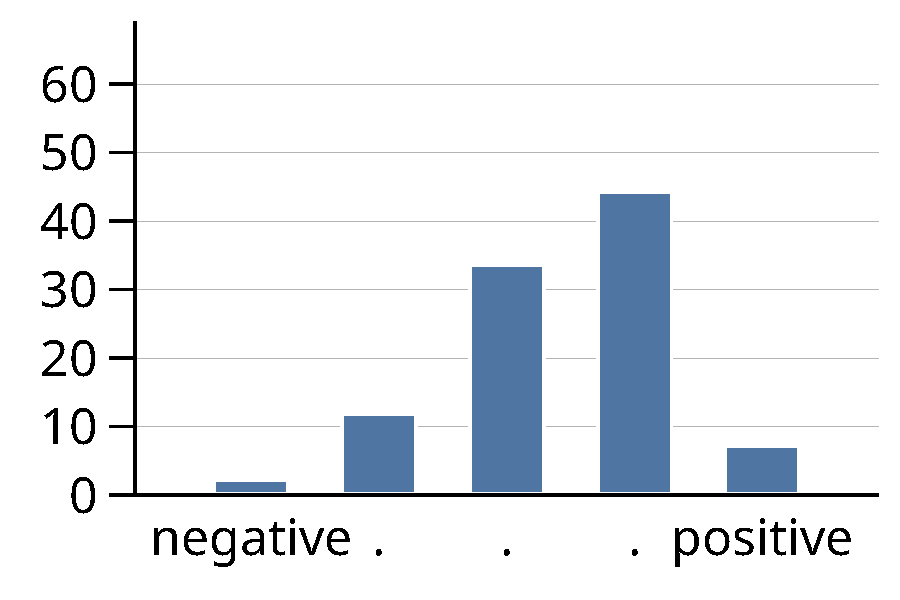
\includegraphics[width=1\linewidth]{descriptives/fig_ment_mh2.pdf}
    \caption{\code{mh2}: Well-balanced in the last 4 weeks}
    \label{fig:mh2}
\end{subfigure}\hfill%
  \begin{subfigure}{.30\textwidth}
    \includegraphics[width=1\linewidth]{descriptives/fig_ment_vt.pdf}
    \caption{\code{vt}: Physical pain in the last 4 weeks}
    \label{fig:vt}
\end{subfigure}\hfill%
  \\  %%%%%%%%%%%%%%%%%%%%%%%%%%%%%%%%%%%%%%%%%%%%%%%%%%%%%%%%%%%%%% newline 
  \begin{subfigure}{.30\textwidth}
    \includegraphics[width=1\linewidth]{descriptives/fig_ment_re1.pdf}
    \caption{\code{re1}: Accomplished less due to emotional problems}
    \label{fig:re1}
\end{subfigure}\hfill%
  \begin{subfigure}{.30\textwidth}
    \includegraphics[width=1\linewidth]{descriptives/fig_ment_re2.pdf}
    \caption{\code{re2}: Less careful due to emotional problems}
    \label{fig:re2}
\end{subfigure}\hfill%
  \begin{subfigure}{.30\textwidth}
    \includegraphics[width=1\linewidth]{descriptives/fig_ment_sf.pdf}
    \caption{\code{sf}: Limited socially due to health \phantom{text}}
    \label{fig:sf}
\end{subfigure}\hfill%
    \caption[Histogram of health variables used in the factor model]
    {Histogram of physical and mental health variables used in the factor model} \par \footnotesize
    \vspace{5pt} 
    Notes: Graphs depict proportion of categories so that they sum up to 100. 
    Labels recoded to order from `negative' to `positive' in terms of health outcome, independently of specific wording.
    For a detailed description on question wording, framing and recoding, see Table~\ref{tab:health_fact_varname_and_questions}.
    \label{fig:main_multifig_phys}
\end{figure}














\begingroup
% The \begingroup ... \endgroup pair ensures values of spacing 
% parameters only affect this particular table, and not any
% subsequent ones in the document.
\renewcommand{\arraystretch}{1.2} % Default value: 1
\renewcommand{\thefootnote}{\alph{footnote}}
\newcommand{\inlinecode}{\texttt}

\newcommand{\rowgroupemph}[1]{\hspace{-1em}\textbf{#1}}
%\newcommand{\rowgroupemph}[1]{\hspace{0em}\underline{#1}}
\begin{table}[tb]
    \centering
    \begin{adjustbox}{max width=.9\textwidth}
        \begin{threeparttable}
            \caption{Overview of module health module from individual questionnaire}
            \label{tab:health_fact_varname_and_questions}
            %\begin{tabularx}{\textwidth}{lX X}
            \begin{tabularx}{\textwidth}{>{\hspace{+1em}}l l >{\raggedright\arraybackslash}X}
                \toprule
                Category            & Variable               & Question \\
                \midrule
                \rowgroupemph{Physical Health Domain} \\ 
                Physical Function 1  & \code{pf1~(ple0004)} & $^{(b)}$When you have to climb several flights of stairs on foot, does your health limit you greatly, somewhat, or not at all?                                                                                      \\
                Physical Function 2  & \code{pf2~(ple0005)} & $^{(b)}$And what about other demanding everyday activities, such as when you have to lift something heavy or do something requiring physical mobility: Does your health limit you greatly, somewhat, or not at all? \\
                General Health       & \code{gh~~(ple0008)} & $^{(c,rev)}$How would you describe your current health?                                                                                                                                                                 \\
                Bodily Pain          & \code{bp~~(ple0030)} & $^{(a)}$have severe physical pain?                                                                                                                                                                                  \\
                Role Physical 1      & \code{rp1~(ple0031)} & $^{(a)}$feel that due to physical health problems you achieved less than you wanted to at work or in everyday activities?                                                                                           \\
                Role Physical 2      & \code{rp2~(ple0032)} & $^{(a)}$feel that due to physical health problems you were limited in some way at work or in everyday activities?                                                                                                   \\[3ex]
                \midrule
                \rowgroupemph{Mental Health Domain} \\
                Stress               & \code{st~~(ple0026)} & $^{(a,e)}$feel rushed or pressed for time?                                                                                                                                                                            \\
                Mental Health 1      & \code{mh1~(ple0027)} & $^{(a)}$feel down and gloomy?                                                                                                                                                                                       \\
                Mental Health 2      & \code{mh2~(ple0028)} & $^{(a,rev)}$feel calm and relaxed?                                                                                                                                                                                      \\
                Vitality             & \code{vt~~(ple0029)} & $^{(a,rev)}$feel energetic?                                                                                                                                                                                             \\
                Role Emotional 1     & \code{re1~(ple0033)} & $^{(a)}$feel that due to mental health or emotional problems you achieved less than you wanted to at work or in everyday activities?                                                                                \\
                Role Emotional 2     & \code{re2~(ple0034)} & $^{(a)}$feel that due to mental health or emotional problems you carried out your work or everyday tasks less thoroughly than usual?                                                                                \\
                Social Function      & \code{sf~~(ple0035)} & $^{(a)}$feel that due to physical or mental health problems you were limited socially, that is, in contact with friends, acquaintances, or relatives?                                                               \\
                \bottomrule
            \end{tabularx}
            %        \begin{tablenotes}[para,flushleft]
                \begin{tablenotes}[para,flushleft]   
                    \footnotesize
                    \item Notes: This table shows an overview of the questions used in the factor models to construct the physical 
                    and mental health scores. Names of input variables from \code{pl} dataset in parenthesis.\\
                    \item a: Categorical variable with 5 levels (1: \textit{Always} to 5: \textit{Never}) and time framed as \textit{previous four weeks}.\\
                    \item b: Categorical variable with 3 levels (1: \textit{Greatly} to 3: \textit{Not at all}) and no explicit time frame.\\
                    \item c: Categorical variable with 5 levels (1: \textit{Very good} to 5: \textit{Bad}) and time framed as \textit{currently}.\\
                    \item rev: Categories order reversed so lower values are `negative' and higher values are `positive' health outcomes.\\
                    \item e: \code{st} is not included SF-12 methodology and, for better comparability, also not in the alternative factor model, but 
                    displayed here for completeness.
                \end{tablenotes}
            \end{threeparttable}
        \end{adjustbox}
    \end{table}
    
    \endgroup













% -------------------------------------------------------------------------------------------------
% Robustness Checks ----
% -------------------------------------------------------------------------------------------------
\chapter{Robustness Checks}

\section{Model specification variation}
\label{modelspecificationvariation}
% -------------------------------------------------------------------------------------------------
% input figures with histograms of mental and physical health questions ----
% -------------------------------------------------------------------------------------------------




\newcommand{\vlgwnlog}{Gross Wealth (log)}                   % gw_nlog
\newcommand{\vlnwnlog}{Net Wealth (neglog)}                  % nw_nlog
\newcommand{\vlgw}{Gross Wealth (k€, winsored)}              % gw
\newcommand{\vlnw}{Net Wealth (k€, winsored)}                % nw
\newcommand{\vlexpue}{Unemployment exp. (months)}            % expue
\newcommand{\vlexpft}{Full-Time exp. (months)}               % expft
\newcommand{\vlemplstatus}{Employment Status of Individual}  % empl_status
\newcommand{\vllaborearns}{Individual Labor Earnings}        % labor_earns
\newcommand{\vlcardioev}{Cardiopathy}                        % cardio_ev
\newcommand{\vldepresev}{Depression}                         % depres_ev


% -------------------------------------------------------------------------------------------------
%  {\vlgwnlog}{Gross Wealth (log)}                   % gw_nlog
% -------------------------------------------------------------------------------------------------
% -------------------------------------------------------------------------------------------------
\begin{figure}[htb!]
    \centering
    \begin{subfigure}{0.45\textwidth}
        \caption{Gross Wealth (log)\qquad Models: P1\tsub{a} / M1\tsub{a}}
        \includegraphics[width=.95\linewidth]{../../output/figures/csdid2/f_robust/ep1_gw_nlog.pdf}
        \label{sfig:ep1_gw_nlog}
    \end{subfigure}
    \begin{subfigure}{0.45\textwidth}
        \caption{Gross Wealth (log)\qquad Models: P1\tsub{b} / M1\tsub{b}}
        \includegraphics[width=.95\linewidth]{../../output/figures/csdid2/f_robust/ep2_gw_nlog.pdf}
        \label{sfig:ep2_gw_nlog}
    \end{subfigure}
    \begin{subfigure}{0.45\textwidth}
        \caption{Gross Wealth (log)\qquad Models: P1\tsub{c} / M1\tsub{c}}
        \includegraphics[width=.95\linewidth]{../../output/figures/csdid2/f_robust/ep3_gw_nlog.pdf}
        \label{sfig:ep3_gw_nlog}
    \end{subfigure}
    \begin{subfigure}{0.45\textwidth}
        \caption{Gross Wealth (log)\qquad Models: P1\tsub{d} / M1\tsub{d}}
        \includegraphics[width=.95\linewidth]{../../output/figures/csdid2/f_robust/ep4_gw_nlog.pdf}
        \label{sfig:ep4_gw_nlog}
    \end{subfigure}
    \caption{Varying model specification}
    \label{fig:ep_gw_nlog}
    \fnote{Notes: Replications with $\log(Gross~Wealth)$ as response variable with  different specifications to check for model dependence.\\
        Models P1\tsub{a} and M1\tsub{a} include not-yet-treated (as well as never-treated) as comparison units. \\ 
        Models P1\tsub{b} and M1\tsub{b} do not include any covariates. \\
        Models P1\tsub{c} and M1\tsub{c} include covariates and are weighted by the inverse probability of remaining in the SOEP, to account for sample attrition might have differential impact over the wealth
        distribution. \\
        Models P1\tsub{d} and M1\tsub{d} are balanced, estimated with people present from 2002 to 2020.
        %                todo: this part to main text body 
        The coefficients are stable across models and similar to those obtained from the 
        main specifications P1 and M1. The estimated coefficients of the mental
        health domain are consistently higher than those of the physical domain. 
        Coefficients (and standard errors) already transformed to represent the effect in percentage terms. 
        The same results are also presented in \cref{tab:t_cmp_gw_nlog}.}
\end{figure}

%S[table-format=1.3, table-space-text-post ={***}]
% -------------------------------------------------------------------------------------------------
%\newcolumntype{p}{>{\columncolor{cp}}S}
%\newcolumntype{P}{>{}S[table-number-alignment = left]}
%\newcolumntype{P}{>{\columncolor{cp}}S[table-number-alignment = left]}
%\newcolumntype{M}{>{\columncolor{cm}}S[table-number-alignment = left]}
\begin{table}[htb!]
    \begin{adjustbox}{max width=\textwidth}
        \begin{threeparttable}
            \scriptsize
            \caption{Varying model specification}
            \label{tab:t_cmp_gw_nlog}
            %            \setlength{\tabcolsep}{12pt}
            \begin{tabular}{l*{4}{P}*{4}{M}}
                \toprule
                & \multicolumn{4}{l}{Physical Health} & \multicolumn{4}{l}{Mental Health}                             \\ %\cmidrule(lr){2-5} \cmidrule(lr){6-9} 
                & \multicolumn{4}{l}{Gross Wealth (log)} & \multicolumn{4}{l}{Gross Wealth (log)}                             \\ \cmidrule(lr){2-5} \cmidrule(lr){6-9} 
                & {(P1\tsub{a})}       & {(P1\tsub{b})}       & {(P1\tsub{c})}        & {(P1\tsub{d})}        & {(M1\tsub{a})}       & {(M1\tsub{b})}       & {(M1\tsub{c})}        & {(M1\tsub{d})}       \\
                & (\%)       & (\%)               & (\%)                & (\%)                & (\%)       & (\%)               & (\%)                &  (\%)              \\
                \midrule%
                
SimpleATT           &      -0.079\sym{**} &      -0.073\sym{**} &      -0.081\sym{***}&      -0.106\sym{*}  &      -0.085\sym{***}&      -0.081\sym{***}&      -0.095\sym{***}&      -0.111\sym{**} \\
                    &      (0.02)         &      (0.02)         &      (0.02)         &      (0.04)         &      (0.02)         &      (0.02)         &      (0.02)         &      (0.04)         \\
Pre\_avg             &       0.026         &       0.031         &       0.009         &       0.048         &       0.020         &       0.005         &      -0.010         &       0.007         \\
                    &      (0.04)         &      (0.04)         &      (0.04)         &      (0.05)         &      (0.03)         &      (0.03)         &      (0.04)         &      (0.05)         \\
Post\_avg            &      -0.090\sym{**} &      -0.089\sym{**} &      -0.099\sym{**} &      -0.111\sym{**} &      -0.107\sym{***}&      -0.101\sym{***}&      -0.116\sym{***}&      -0.113\sym{**} \\
                    &      (0.03)         &      (0.03)         &      (0.03)         &      (0.04)         &      (0.03)         &      (0.03)         &      (0.03)         &      (0.04)         \\
tm10                &      -0.012         &       0.013         &      -0.014         &       0.040         &       0.034         &       0.020         &      -0.038         &       0.111         \\
                    &      (0.09)         &      (0.09)         &      (0.09)         &      (0.10)         &      (0.07)         &      (0.07)         &      (0.08)         &      (0.09)         \\
tm8                 &       0.068         &       0.073         &       0.033         &       0.074         &       0.004         &      -0.025         &      -0.030         &      -0.048         \\
                    &      (0.05)         &      (0.05)         &      (0.06)         &      (0.07)         &      (0.05)         &      (0.05)         &      (0.05)         &      (0.07)         \\
tm6                 &       0.013         &       0.007         &      -0.016         &       0.032         &       0.010         &      -0.002         &       0.004         &      -0.036         \\
                    &      (0.04)         &      (0.04)         &      (0.04)         &      (0.05)         &      (0.03)         &      (0.03)         &      (0.04)         &      (0.05)         \\
tm4                 &       0.034\sym{*}  &       0.031\sym{*}  &       0.032\sym{*}  &       0.044         &       0.031\sym{*}  &       0.028         &       0.025         &       0.000         \\
                    &      (0.02)         &      (0.02)         &      (0.02)         &      (0.02)         &      (0.02)         &      (0.01)         &      (0.02)         &      (0.03)         \\
tp0                 &      -0.022         &      -0.014         &      -0.021         &      -0.033         &      -0.011         &      -0.010         &      -0.022         &      -0.028         \\
                    &      (0.01)         &      (0.01)         &      (0.01)         &      (0.02)         &      (0.01)         &      (0.01)         &      (0.01)         &      (0.02)         \\
tp2                 &      -0.038\sym{*}  &      -0.026         &      -0.036         &      -0.073\sym{*}  &      -0.032         &      -0.031         &      -0.046\sym{*}  &      -0.049         \\
                    &      (0.02)         &      (0.02)         &      (0.02)         &      (0.03)         &      (0.02)         &      (0.02)         &      (0.02)         &      (0.03)         \\
tp4                 &      -0.099\sym{***}&      -0.095\sym{***}&      -0.099\sym{***}&      -0.099\sym{*}  &      -0.102\sym{***}&      -0.103\sym{***}&      -0.118\sym{***}&      -0.090\sym{*}  \\
                    &      (0.03)         &      (0.03)         &      (0.03)         &      (0.04)         &      (0.03)         &      (0.02)         &      (0.03)         &      (0.04)         \\
tp6                 &      -0.133\sym{***}&      -0.118\sym{***}&      -0.126\sym{***}&      -0.133\sym{**} &      -0.122\sym{***}&      -0.114\sym{***}&      -0.130\sym{***}&      -0.120\sym{**} \\
                    &      (0.04)         &      (0.03)         &      (0.04)         &      (0.05)         &      (0.03)         &      (0.03)         &      (0.03)         &      (0.05)         \\
tp8                 &      -0.148\sym{***}&      -0.136\sym{**} &      -0.147\sym{**} &      -0.136\sym{*}  &      -0.169\sym{***}&      -0.150\sym{***}&      -0.167\sym{***}&      -0.166\sym{**} \\
                    &      (0.04)         &      (0.04)         &      (0.05)         &      (0.06)         &      (0.04)         &      (0.04)         &      (0.04)         &      (0.05)         \\
tp10                &      -0.111\sym{*}  &      -0.131\sym{**} &      -0.148\sym{**} &      -0.177\sym{**} &      -0.125\sym{**} &      -0.122\sym{**} &      -0.139\sym{**} &      -0.161\sym{**} \\
                    &      (0.05)         &      (0.05)         &      (0.05)         &      (0.06)         &      (0.05)         &      (0.04)         &      (0.05)         &      (0.06)         \\
tp12                &      -0.081         &      -0.103         &      -0.114         &      -0.127         &      -0.187\sym{**} &      -0.176\sym{***}&      -0.188\sym{***}&      -0.178\sym{**} \\
                    &      (0.07)         &      (0.06)         &      (0.07)         &      (0.07)         &      (0.06)         &      (0.05)         &      (0.06)         &      (0.06)         \\
\midrule
Pretrend $\chi^2$ (df)&       26.71         &       28.00         &       22.61         &       36.19         &       16.45         &       19.18         &       20.14         &       65.88         \\
Pretrend p-value    &  22 (0.222)         &  22 (0.176)         &  22 (0.424)         &  28 (0.138)         &  22 (0.793)         &  22 (0.634)         &  22 (0.574)         &  28 (0.000)         \\
Covariates          &                     &$\checkmark$         &$\checkmark$         &$\checkmark$         &                     &$\checkmark$         &$\checkmark$         &$\checkmark$         \\
Inv.Pr(stay)        &                     &                     &$\checkmark$         &                     &                     &                     &$\checkmark$         &                     \\
Balanced            &                     &                     &                     &$\checkmark$         &                     &                     &                     &$\checkmark$         \\
\bottomrule

            \end{tabular}
            \begin{tablenotes}[para,flushleft]
                \vspace*{-\baselineskip} {\raggedleft*~$p<0.05$,~**~$p<0.01$,~***~$p<0.001$\\}
                Notes: Replications with $\log(Gross~Wealth)$ as response variable with different specifications to check for model dependence.  
                Wild Bootstrap standard error in parenthesis. 
                \item Models P1\tsub{a} and M1\tsub{a} include not-yet-treated (as well as never-treated) as comparison units. \\ 
                \item Models P1\tsub{b} and M1\tsub{b} do not include any covariates. \\
                \item Models P1\tsub{c} and M1\tsub{c} include covariates and are weighted by the inverse probability of remaining in the SOEP, to account for sample attrition might have differential impact over the wealth
                distribution. \\
                \item Models P1\tsub{d} and M1\tsub{d} are balanced, estimated with people present from 2002 to 2020.
                %                todo: this part to main text body 
                The coefficients are stable across models and similar to those obtained from the 
                main specifications P1 and M1. 
                The covariates included are gender, age spline, federal state residence, legal disability, marital status, and years of education.
                Coefficients (and standard errors) already transformed to represent the effect in percentage terms. 
                For a visual representation of the same results see \cref{fig:ep_gw_nlog}.
            \end{tablenotes}
        \end{threeparttable}
    \end{adjustbox}
\end{table} % todo: include number in balanced model
% -------------------------------------------------------------------------------------------------
% -------------------------------------------------------------------------------------------------



% -------------------------------------------------------------------------------------------------
% tab:diff_treat_rule ----
% -------------------------------------------------------------------------------------------------
\begin{table}[htbp!]
    \centering \
    \begin{adjustbox}{max width=1\textwidth}
        \begin{threeparttable}
            \scriptsize
            \caption{Table of results with different treatment rule}
            \label{tab:diff_treat_rule}
            \setlength{\tabcolsep}{6pt}
            \begin{tabular}{l PPPP MMMM}
                \toprule
                & \multicolumn{4}{l}{Physical Health} & \multicolumn{4}{l}{Mental Health}                             \\ \cmidrule(lr){2-5} \cmidrule(lr){6-9} 
                & \multicolumn{2}{l}{(neg)log} & \multicolumn{2}{l}{level} & \multicolumn{2}{l}{(neg)log} & \multicolumn{2}{l}{level} \\ \cmidrule(lr){2-3} \cmidrule(lr){4-5} \cmidrule(lr){6-7} \cmidrule(lr){8-9} 
                & {gross (\%)} & {net (\%)$^1$} & {gross} & {net} & {gross (\%)} & {net (\%)$^1$} & {gross} & {net}           \\ 
                & {(P1\tsub{r})}       & {(P2\tsub{r})}       & {(P3\tsub{r})}        & {(P4\tsub{r})}        & {(M1\tsub{r})}       & {(M2\tsub{r})}       & {(M3\tsub{r})}        & {(M4\tsub{r})}       \\
                \midrule%
                
SimpleATT           &       -3.44\sym{*}  &       -2.77         &       -4.07\sym{*}  &       -4.47\sym{**} &       -7.36\sym{***}&       -8.40\sym{***}&       -4.52\sym{*}  &       -3.97\sym{*}  \\
                    &      (1.70)         &      (2.39)         &      (1.75)         &      (1.56)         &      (1.62)         &      (2.13)         &      (1.80)         &      (1.62)         \\
Pre average             &        1.60         &        4.74         &        3.47         &        2.86         &        3.00         &        4.75         &        1.53         &        2.16         \\
                    &      (2.24)         &      (3.41)         &      (2.12)         &      (1.92)         &      (2.42)         &      (3.12)         &      (2.73)         &      (2.26)         \\
Post average            &       -4.80         &       -3.25         &       -6.47\sym{*}  &       -6.75\sym{**} &       -9.66\sym{***}&      -10.74\sym{***}&       -6.37\sym{*}  &       -5.39\sym{*}  \\
                    &      (2.49)         &      (3.63)         &      (2.70)         &      (2.44)         &      (2.17)         &      (2.91)         &      (2.83)         &      (2.31)         \\
$\hat{\theta}_{es}(-10)$                &        6.04         &        9.38         &        5.62         &        5.11         &        3.22         &        5.53         &        1.15         &        3.89         \\
                    &      (4.67)         &      (7.28)         &      (4.00)         &      (3.72)         &      (5.05)         &      (6.71)         &      (5.40)         &      (4.76)         \\
$\hat{\theta}_{es}(-8)$                 &       -1.76         &        1.73         &        2.80         &        1.86         &        4.50         &        7.53         &        1.98         &        3.48         \\
                    &      (3.27)         &      (4.85)         &      (3.20)         &      (2.86)         &      (3.47)         &      (4.81)         &      (3.54)         &      (3.12)         \\
$\hat{\theta}_{es}(-6)$                 &        1.22         &        4.12         &        4.64\sym{*}  &        3.57\sym{*}  &        2.41         &        1.66         &        1.46         &        0.19         \\
                    &      (2.09)         &      (3.04)         &      (1.97)         &      (1.71)         &      (2.10)         &      (2.89)         &      (2.22)         &      (2.03)         \\
$\hat{\theta}_{es}(-4)$                 &        1.03         &        3.86\sym{*}  &        0.81         &        0.88         &        1.90         &        4.37\sym{**} &        1.54         &        1.09         \\
                    &      (1.12)         &      (1.63)         &      (0.95)         &      (0.86)         &      (1.13)         &      (1.50)         &      (0.97)         &      (0.86)         \\
$\hat{\theta}_{es}(0)$                 &       -0.69         &       -2.45         &       -0.77         &       -1.19         &       -2.41\sym{**} &       -2.76\sym{*}  &       -1.79\sym{*}  &       -1.36\sym{*}  \\
                    &      (0.77)         &      (1.34)         &      (0.74)         &      (0.73)         &      (0.80)         &      (1.16)         &      (0.71)         &      (0.69)         \\
$\hat{\theta}_{es}(2)$                 &       -2.56         &       -3.19         &       -3.42\sym{*}  &       -3.46\sym{*}  &       -4.14\sym{**} &       -5.10\sym{*}  &       -2.53         &       -2.49         \\
                    &      (1.58)         &      (2.50)         &      (1.51)         &      (1.39)         &      (1.53)         &      (2.28)         &      (1.51)         &      (1.42)         \\
$\hat{\theta}_{es}(4)$                 &       -3.94         &       -1.41         &       -4.77\sym{*}  &       -6.06\sym{**} &      -10.91\sym{***}&      -12.36\sym{***}&       -5.25\sym{*}  &       -5.30\sym{**} \\
                    &      (2.26)         &      (3.73)         &      (2.35)         &      (2.17)         &      (2.07)         &      (2.96)         &      (2.37)         &      (2.02)         \\
$\hat{\theta}_{es}(6)$                 &       -6.21\sym{*}  &       -3.57         &       -4.72         &       -5.79\sym{*}  &      -11.42\sym{***}&      -14.55\sym{***}&       -7.17\sym{*}  &       -6.24\sym{*}  \\
                    &      (2.79)         &      (4.39)         &      (2.93)         &      (2.51)         &      (2.46)         &      (3.35)         &      (3.01)         &      (2.78)         \\
$\hat{\theta}_{es}(8)$                 &       -7.76\sym{*}  &       -2.10         &       -6.49         &       -5.63         &      -13.42\sym{***}&      -14.26\sym{**} &       -7.64\sym{*}  &       -6.91\sym{*}  \\
                    &      (3.55)         &      (5.35)         &      (3.87)         &      (3.50)         &      (3.08)         &      (4.23)         &      (3.89)         &      (3.39)         \\
$\hat{\theta}_{es}(10)$                &       -5.71         &       -3.02         &      -10.44\sym{*}  &      -10.35\sym{*}  &      -12.58\sym{**} &      -11.91\sym{*}  &       -7.71         &       -6.59         \\
                    &      (4.18)         &      (6.35)         &      (5.29)         &      (4.45)         &      (3.95)         &      (4.91)         &      (5.20)         &      (4.63)         \\
$\hat{\theta}_{es}(12)$                &       -6.51         &       -6.88         &      -14.66\sym{*}  &      -14.77\sym{*}  &      -12.13\sym{*}  &      -13.50\sym{*}  &      -12.48         &       -8.83         \\
                    &      (6.02)         &      (7.54)         &      (6.82)         &      (5.94)         &      (4.74)         &      (6.13)         &      (6.52)         &      (5.44)         \\
\midrule
Obs                 &       90207         &       90207         &       90207         &       90207         &       84925         &       84925         &       84925         &       84925         \\
Pretrend $\chi^2$ (df)&  24.83 (26)         &  18.10 (26)         &  36.22 (26)         &  38.92 (26)         &  23.44 (26)         &  29.88 (26)         &  36.60 (26)         &  31.64 (26)         \\
Pretrend p-value    &       0.529         &       0.872         &       0.088         &       0.050         &       0.608         &       0.272         &       0.081         &       0.205         \\
\bottomrule

            \end{tabular}
            \begin{tablenotes}[para,flushleft]
                \vspace*{-\baselineskip} 
                {\raggedleft*~$p<0.05$,~**~$p<0.01$,~***~$p<0.001$ \\}
                Notes: Results of replicating the primary model with a different assignment rule. 
                Instead of having to experience a negative health outcome at least twice, people experiencing it 
                only once is already assigned to treatment. Further, the threshold is 1~Std.~Dev. instead of $1/2$ used in the main analysis. 
                In general, the results are similar, but consistently smaller than in the main analysis. The difference is
                around half to two thirds of estimations in the main results. The only model which is not strongly affected
                by these parameter changes is the one with gross wealth in logarithms as the response variable, M1\tsub{r} in the
                robustness checks and M1 in the main analysis. 
                The covariates included are gender, age spline, federal state residence, legal disability, marital status, and years of education.
                $^1$Coefficients (and standard errors) of log specifications are transformed to represent the effect in percentage terms, but
                such interpretation of the neglog transformation might be biased (see \cref{sec:transformcoefs})
                Wild Bootstrap standard error in parenthesis. 
                The main results are presented in \cref{tab:main_res_event} and the corresponding notes 
                on the procedure apply to this table equally. 
            \end{tablenotes}
        \end{threeparttable}
    \end{adjustbox}
\end{table}
% -------------------------------------------------------------------------------------------------
% -------------------------------------------------------------------------------------------------





% -------------------------------------------------------------------------------------------------
% figure: robustness checks (diff treat rule) ----
% -------------------------------------------------------------------------------------------------
\begin{figure}[ht!]
    \centering
    \begin{subfigure}{0.45\textwidth}
        \caption{Gross Wealth (log)\\(P1\tsub{r} / M1\tsub{r})}
        \includegraphics[width=.95\linewidth]{../../output/figures/csdid2/b_mcspcs/f_11_gw_nlog_1_ct1.pdf}
        \label{sfig:did_gw_nlog1ct1}
    \end{subfigure}
    \begin{subfigure}{0.45\textwidth}
        \caption{Net Wealth (neglog)\\(P2\tsub{r} / M2\tsub{r})}
        \includegraphics[width=.95\linewidth]{../../output/figures/csdid2/b_mcspcs/f_21_nw_nlog_1_ct1.pdf}
        \label{sfig:did_nw_nlog1ct1}
    \end{subfigure}
    \begin{subfigure}{0.45\textwidth}
        \caption{Gross Wealth (k€, winsored)\\(P3\tsub{r} / M3\tsub{r})}
        \includegraphics[width=.95\linewidth]{../../output/figures/csdid2/b_mcspcs/f_31_gw_1_ct1.pdf}
        \label{sfig:did_gw1ct1}
    \end{subfigure}
    \begin{subfigure}{0.45\textwidth}
        \caption{Net Wealth (k€, winsored)\\(P4\tsub{r} / M4\tsub{r})}
        \includegraphics[width=.95\linewidth]{../../output/figures/csdid2/b_mcspcs/f_41_nw_1_ct1.pdf}
        \label{sfig:did_nw1ct1}
    \end{subfigure}
    \caption{Event-study results with different treatment assignment rule}
    \label{fig:diff_treat_rule}
    \fnote{Notes: The results corresponding to this panel is presented in \cref{tab:diff_treat_rule}.
        The same notes apply to this figure. }
\end{figure}



% pcs_main        // Physical Health (oblique)
% gw_nlog         // Gross Wealth (log)
% gw              // Gross Wealth (k€, winsored)
% pcs_main        // Physical Health (oblique)
% empl_status     // Employment Status of Individual
% sats_health     // Satisfaction With Health
% mcs_main        // Mental Health (oblique)
% gw_nlog         // Gross Wealth (log)
% gw              // Gross Wealth (k€, winsored)
% mcs_main        // Mental Health (oblique)
% expue           // Unemployment exp. (months)
% sats_health     // Satisfaction With Health




\begin{figure}[htb!]
    % -------------------------------------------------------------------------------------------------
    % var: pcs_main         % Physical Health Domain
    % -------------------------------------------------------------------------------------------------
    % -------------------------------------------------------------------------------------------------
    \centering \setcounter{subfigure}{0}% Reset subfigure counter
    %%A: Physical Health Domain
    %\\ %%%%%%%%%%%%%%%%%%%%%%%%%%%%%%%%%%%%%%%%%%%%%%%%%%%%%%%%%%%%%%%%%%%%%%%%%%%%%%%%%%%%%%%%%%%
    \begin{subfigure}{0.32\textwidth}
        \caption{Physical Health (oblique)}
        \includegraphics[width=.95\linewidth]{../../output/figures/csdid2/h_descr/f_pcs_main_pcs_main_n1_win1.pdf}
        \label{sfig:fpcsmainpcsmain}
    \end{subfigure}
    \begin{subfigure}{0.32\textwidth}
        \caption{Gross Wealth (log)}
        \includegraphics[width=.95\linewidth]{../../output/figures/csdid2/h_descr/f_gw_nlog_pcs_main_n1_win1.pdf}
        \label{sfig:fgwnlogpcsmain}
    \end{subfigure}
    \begin{subfigure}{0.32\textwidth}
        \caption{Gross Wealth (k€, winsored)}
        \includegraphics[width=.95\linewidth]{../../output/figures/csdid2/h_descr/f_gw_pcs_main_n1_win1.pdf}
        \label{sfig:fgwpcsmain}
    \end{subfigure}
    \begin{subfigure}{0.32\textwidth}
        \caption{Mental Health (oblique)}
        \includegraphics[width=.95\linewidth]{../../output/figures/csdid2/h_descr/f_pcs_main_mcs_main_n1_win1.pdf}
        \label{sfig:fpcsmainmcsmain}
    \end{subfigure}
    \begin{subfigure}{0.32\textwidth}
        \caption{Unemployment exp. (months)}
        \includegraphics[width=.95\linewidth]{../../output/figures/csdid2/h_descr/f_expue_pcs_main_n1_win1.pdf}
        \label{sfig:fexpuepcsmain}
    \end{subfigure}
    \begin{subfigure}{0.32\textwidth}
        \caption{Satisfaction With Health}
        \includegraphics[width=.95\linewidth]{../../output/figures/csdid2/h_descr/f_sats_health_pcs_main_n1_win1.pdf}
        \label{sfig:fsatshealthpcsmain}
    \end{subfigure}
    % start main caption
    \caption{Development of selected variables from event study (Physical Health Domain)}
    \label{fig:inlevelspcsmain}
    \fnote{Panels depict the evolution of selected variables for the
        treated group (in red) and the untreated (in blue). In panel (a), one can see that, on average, the untreated do experience a strong direct impact at $e=0$
        but it recovers to the previous values in the next period ($e=2$), while the treated recovers only
        slightly and carry on on a downward trend. In panel (d), one can see the cross effect on the other health domain. That is,
        how does the shock in the one health dimension affect the other health dimension. Whiskers depict the 99\% confidence interval. \\
        Notes:\\
        - a: The untreated group, by definition, are not
        assigned a ``event year'', so their event is set as the year when they experience their worst
        health outcome, albeit still below the threshold. The actual DiD procedure do not impute any treatment
        year for the untreated, but for this visualization, one has to set a date or assign randomly and any
        choice would have some drawbacks. This choice is able depicting the evolution of people on limit of treatment assignment.\\
        - b: The vertical line depict the last period before (imputed) treatment taking place.\\
        - c: To avoid sample composition affecting the interpretation of these figures, the sample is restricted to a balanced panel.}
\end{figure}

\begin{figure}[htb!]
    % -------------------------------------------------------------------------------------------------
    % var: mcs_main         % Mental Health Domain
    % -------------------------------------------------------------------------------------------------
    % -------------------------------------------------------------------------------------------------
    \centering \setcounter{subfigure}{0}% Reset subfigure counter
    %%A: Mental Health Domain
    %\\ %%%%%%%%%%%%%%%%%%%%%%%%%%%%%%%%%%%%%%%%%%%%%%%%%%%%%%%%%%%%%%%%%%%%%%%%%%%%%%%%%%%%%%%%%%%
    \begin{subfigure}{0.32\textwidth}
        \caption{Mental Health (oblique)}
        \includegraphics[width=.95\linewidth]{../../output/figures/csdid2/h_descr/f_mcs_main_mcs_main_n1_win1.pdf}
        \label{sfig:fmcsmainmcsmain}
    \end{subfigure}
    \begin{subfigure}{0.32\textwidth}
        \caption{Gross Wealth (log)}
        \includegraphics[width=.95\linewidth]{../../output/figures/csdid2/h_descr/f_gw_nlog_mcs_main_n1_win1.pdf}
        \label{sfig:fgwnlogmcsmain}
    \end{subfigure}
    \begin{subfigure}{0.32\textwidth}
        \caption{Gross Wealth (k€, winsored)}
        \includegraphics[width=.95\linewidth]{../../output/figures/csdid2/h_descr/f_gw_mcs_main_n1_win1.pdf}
        \label{sfig:fgwmcsmain}
    \end{subfigure}
    \begin{subfigure}{0.32\textwidth}
        \caption{Physical Health (oblique)}
        \includegraphics[width=.95\linewidth]{../../output/figures/csdid2/h_descr/f_mcs_main_pcs_main_n1_win1.pdf}
        \label{sfig:fmcsmainpcsmain}
    \end{subfigure}
    \begin{subfigure}{0.32\textwidth}
        \caption{Unemployment exp. (months)}
        \includegraphics[width=.95\linewidth]{../../output/figures/csdid2/h_descr/f_expue_mcs_main_n1_win1.pdf}
        \label{sfig:fexpuemcsmain}
    \end{subfigure}
    \begin{subfigure}{0.32\textwidth}
        \caption{Satisfaction With Health}
        \includegraphics[width=.95\linewidth]{../../output/figures/csdid2/h_descr/f_sats_health_mcs_main_n1_win1.pdf}
        \label{sfig:fsatshealthmcsmain}
    \end{subfigure}
    % start main caption
    \caption{Development of selected variables from event study (Mental Health Domain)}
    \label{fig:inlevelsmcsmain}
    \fnote{Notes: points a: b: and c: of \cref{fig:inlevelspcsmain} also apply, as well as similar interpretation of each panels.
        Emphasis here to panel (e), showing a nice example of the effect taking place after not only parallel but equal pre-trend.}
\end{figure}



\begin{figure}
    \centering
    {Kaplan--Meier survival estimates}\par
    \includegraphics[width=0.7\linewidth]{../../output/figures/attrition/kpme_surv_nw_qile_age}
    \caption{Survival analysis of SOEP participants by wealth quintiles}
    \label{fig:kpmesurvnwqileage}
    \fnote{
        Notes: This graph evidentiates the gradient in panel attrition by wealth levels.
        It depicts an unadjusted survival estimate of participation length for each quintile of 
        age-adjusted gross wealth.  While the four upper quintile groups show a similar survival rate, 
        those in the bottom quintile are less likely to remain as long in the SOEP.
        The graph suggests that the differential attrition 
        rate is stronger in the first 5 years. From then on, the curves evolve parallel to one another. 
        For this analysis, SOEP's entering yeard is used, including if it happened before 2002. Those that dropped out
        before 2002 (from when on wealth data are available) are not considered for this examination. 
        Data source: SOEPv37.
        }
\end{figure}






% -------------------------------------------------------------------------------------------------
% -------------------------------------------------------------------------------------------------
% -------------------------------------------------------------------------------------------------
% -------------------------------------------------------------------------------------------------
% PCS_DEF ----
\chapter{Replications based on the SF-12 method}%
%
% -------------------------------------------------------------------------------------------------
% -------------------------------------------------------------------------------------------------
% -------------------------------------------------------------------------------------------------
\begin{figure}
    % -------------------------------------------------------------------------------------------------
    % var: pcs_def         % Physical Health Domain
    % -------------------------------------------------------------------------------------------------
    % -------------------------------------------------------------------------------------------------
    \centering \setcounter{subfigure}{0}% Reset subfigure counter
    \renewcommand{\thesubfigure}{P\alph{subfigure}}
    Physical Health Domain
    \\ %%%%%%%%%%%%%%%%%%%%%%%%%%%%%%%%%%%%%%%%%%%%%%%%%%%%%%%%%%%%%%%%%%%%%%%%%%%%%%%%%%%%%%%%%%%
    \begin{subfigure}{0.32\textwidth}
        \caption{Physical Health (oblique)}
        \includegraphics[width=.95\linewidth]{../../output/figures/csdid2/h_descr/f_pcs_def_pcs_def_n1_win1.pdf}
        \label{sfig:fpcsdefpcsdef}
    \end{subfigure}
    \begin{subfigure}{0.32\textwidth}
        \caption{Gross Wealth (log)}
        \includegraphics[width=.95\linewidth]{../../output/figures/csdid2/h_descr/f_gw_nlog_pcs_def_n1_win1.pdf}
        \label{sfig:fgwnlogpcsdef}
    \end{subfigure}
    \begin{subfigure}{0.32\textwidth}
        \caption{Gross Wealth (k€, winsored)}
        \includegraphics[width=.95\linewidth]{../../output/figures/csdid2/h_descr/f_gw_pcs_def_n1_win1.pdf}
        \label{sfig:fgwpcsdef}
    \end{subfigure}
    \begin{subfigure}{0.32\textwidth}
        \caption{Mental Health (oblique)}
        \includegraphics[width=.95\linewidth]{../../output/figures/csdid2/h_descr/f_pcs_def_mcs_def_n1_win1.pdf}
        \label{sfig:fpcsdefmcsdef}
    \end{subfigure}
    \begin{subfigure}{0.32\textwidth}
        \caption{Unemployment exp. (months)}
        \includegraphics[width=.95\linewidth]{../../output/figures/csdid2/h_descr/f_expue_pcs_def_n1_win1.pdf}
        \label{sfig:fexpuepcsdef}
    \end{subfigure}
    \begin{subfigure}{0.32\textwidth}
        \caption{Satisfaction With Health}
        \includegraphics[width=.95\linewidth]{../../output/figures/csdid2/h_descr/f_sats_health_pcs_def_n1_win1.pdf}
        \label{sfig:fsatshealthpcsdef}
    \end{subfigure}
%    % start def caption
%    \caption{Development of selected variables from event study (Physical Health Domain)}
%    \label{fig:inlevelspcsdef}
%    \fnote{}
%\end{figure}
%\begin{figure}[htb!]
%    % -------------------------------------------------------------------------------------------------
%    % var: mcs_def         % Mental Health Domain
%    % -------------------------------------------------------------------------------------------------
%    % -------------------------------------------------------------------------------------------------
    \centering \setcounter{subfigure}{0}% Reset subfigure counter
    \renewcommand{\thesubfigure}{M\alph{subfigure}}
    Mental Health Domain
    \\ %%%%%%%%%%%%%%%%%%%%%%%%%%%%%%%%%%%%%%%%%%%%%%%%%%%%%%%%%%%%%%%%%%%%%%%%%%%%%%%%%%%%%%%%%%%
    \begin{subfigure}{0.32\textwidth}
        \caption{Mental Health (oblique)}
        \includegraphics[width=.95\linewidth]{../../output/figures/csdid2/h_descr/f_mcs_def_mcs_def_n1_win1.pdf}
        \label{sfig:fmcsdefmcsdef}
    \end{subfigure}
    \begin{subfigure}{0.32\textwidth}
        \caption{Gross Wealth (log)}
        \includegraphics[width=.95\linewidth]{../../output/figures/csdid2/h_descr/f_gw_nlog_mcs_def_n1_win1.pdf}
        \label{sfig:fgwnlogmcsdef}
    \end{subfigure}
    \begin{subfigure}{0.32\textwidth}
        \caption{Gross Wealth (k€, winsored)}
        \includegraphics[width=.95\linewidth]{../../output/figures/csdid2/h_descr/f_gw_mcs_def_n1_win1.pdf}
        \label{sfig:fgwmcsdef}
    \end{subfigure}
    \begin{subfigure}{0.32\textwidth}
        \caption{Physical Health (oblique)}
        \includegraphics[width=.95\linewidth]{../../output/figures/csdid2/h_descr/f_mcs_def_pcs_def_n1_win1.pdf}
        \label{sfig:fmcsdefpcsdef}
    \end{subfigure}
    \begin{subfigure}{0.32\textwidth}
        \caption{Unemployment exp. (months)}
        \includegraphics[width=.95\linewidth]{../../output/figures/csdid2/h_descr/f_expue_mcs_def_n1_win1.pdf}
        \label{sfig:fexpuemcsdef}
    \end{subfigure}
    \begin{subfigure}{0.32\textwidth}
        \caption{Satisfaction With Health}
        \includegraphics[width=.95\linewidth]{../../output/figures/csdid2/h_descr/f_sats_health_mcs_def_n1_win1.pdf}
        \label{sfig:fsatshealthmcsdef}
    \end{subfigure}
    % start main caption
    \caption{Development of selected variables based on SF-12 method}
    \label{fig:inlevelsmcsdef}
    \fnote{Notes: Replication of \cref{fig:inlevelspcsmain,fig:inlevelsmcsmain} using PCS and MCS following the SF-12 method.
    Here one can observe the negative cross-effect in \subref{sfig:fpcsdefmcsdef} and \subref{sfig:fmcsdefpcsdef} where the adverse outcome 
    in one dimension impacts the other dimension in the opposite direction. The pre-treatment trend, specially in \subref{sfig:fexpuepcsdef} 
    and \subref{sfig:fexpuemcsdef}, are less supportive of the parallel trends assumption than in the alternative method.
    Same considerations regarding the ``treatment date'' of the untreated stated in the notes of  \cref{fig:inlevelspcsmain} apply here as well.}
\end{figure}





% ---------------------------------------------------------------------------------------------------------------------
% Validation with objective health diagnoses
% ---------------------------------------------------------------------------------------------------------------------
\begin{figure}[tb!]
    \centering
    \begin{subfigure}{0.45\textwidth}
        \caption{Depression}
        \includegraphics[width=.95\linewidth]{../../output/figures/csdid2/c_othervars/f_2_depres_ev_1o2_def.pdf}
    \end{subfigure}
    \begin{subfigure}{0.45\textwidth}
        \caption{Sleep Disorder}
        \includegraphics[width=.95\linewidth]{../../output/figures/csdid2/c_othervars/f_2_sleep_ev_1o2_def.pdf}
    \end{subfigure}
    \caption{Replication of validation of mental health diagnoses with orthogonal health scores} 
    \label{fig:csdid_hltdiag_rep}
    \fnote{Notes: This replication aims to show that also using orthogonal health scores, the effect follows 
        a similar in both domains, similar to using oblique scores. 
        Response variables are binary indicators of being ever diagnosed with the respective condition.
        Panels have different scale on the y-axis. Whiskers depict the 95\% confidence interval}
\end{figure}








































% -------------------------------------------------------------------------------------------------
% figure: SF-12 default pcs mcs
% -------------------------------------------------------------------------------------------------
\begin{figure}[ht!]
    \centering
    \begin{subfigure}{0.45\textwidth}
        \caption{Gross Wealth (log)\\(M1\tsub{sf12} / P1\tsub{sf12})}
        \includegraphics[width=.95\linewidth]{../../output/figures/csdid2/b_mcspcs/f_12_gw_nlog_1o2_ct2.pdf}
        \label{sfig:did_sf12_a}
    \end{subfigure}
    \begin{subfigure}{0.45\textwidth}
        \caption{Net Wealth (neglog)\\(M2\tsub{sf12} / P2\tsub{sf12})}
        \includegraphics[width=.95\linewidth]{../../output/figures/csdid2/b_mcspcs/f_22_nw_nlog_1o2_ct2.pdf}
        \label{sfig:did_sf12_b}
    \end{subfigure}
    \begin{subfigure}{0.45\textwidth}
        \caption{Gross Wealth (k€, winsored)\\(M3\tsub{sf12} / P3\tsub{sf12})}
        \includegraphics[width=.95\linewidth]{../../output/figures/csdid2/b_mcspcs/f_32_gw_1o2_ct2.pdf}
        \label{sfig:did_sf12_c}
    \end{subfigure}
    \begin{subfigure}{0.45\textwidth}
        \caption{Net Wealth (k€, winsored)\\(M4\tsub{sf12} / P4\tsub{sf12})}
        \includegraphics[width=.95\linewidth]{../../output/figures/csdid2/b_mcspcs/f_42_nw_1o2_ct2.pdf}
        \label{sfig:did_sf12_d}
    \end{subfigure}
    \caption{Replication of main analysis with SF-12 scores}
    \label{fig:did_sf12}
    \fnote{Notes: These panels are a visual representation of the table of coefficients presented in \cref{tab:coefs_sf12}. 
        Post-treatment, the effects are in line with those obtained in the main analysis. Pre-treatment, in contrast, seems 
        to be less supportive of the parallel trends assumptions, including in the primary specifications with log-transformed 
        gross wealth (P1\tsub{sf12} and M1\tsub{sf12}). To what extend this is driven by the particular treatment rule or
        whether an artifact from the sf12 or from the alternative scores computes could be a matter of further inquiry.
        To what extend should be, a priori, expected that the trends remain parallel 8 or 10 years prior to treatment 
        is also worth considering. 
    Whiskers depict the 95\% confidence interval.}
\end{figure}



\begin{table}[htbp!]
    \centering
    \begin{adjustbox}{max width=\textwidth}
        \begin{threeparttable}       
            \caption{Table of coefficients of models based on the SF-12 methodology}
            \label{tab:coefs_sf12} % \setlength{\tabcolsep}{4pt}
            \begin{tabular}{l*4{P}*4{M}}
                \toprule
                & \multicolumn{4}{l}{Physical Health}   & \multicolumn{4}{l}{Mental Health}     \\ \cmidrule(lr{1em}){2-5} \cmidrule(lr{1em}){6-9}
                & \multicolumn{2}{l}{(neg)log}               & \multicolumn{2}{l}{level} & \multicolumn{2}{l}{(neg)log} & \multicolumn{2}{l}{level} \\ \cmidrule(lr{1em}){2-3} \cmidrule(lr{1em}){4-5} \cmidrule(lr{1em}){6-7} \cmidrule(lr{1em}){8-9} 
                & {gross (\%)} & {net (\%)$^1$} & {gross} & {net} & {gross (\%)} & {net (\%)$^1$} & {gross} & {net}               \\
                & {(P1\tsub{sf12})}  & {(P2\tsub{sf12})}            & {(P3\tsub{sf12})}  & {(P4\tsub{sf12})}              & {(M1\tsub{sf12})}  & {(M2\tsub{sf12})}            & {(M3\tsub{sf12})}  & {(M4\tsub{sf12})}              \\  
                \midrule
                \input{./incl/tbls/tbl_full_def_bd_1o2_ct2.tex}% &
            \end{tabular}%
            \begin{tablenotes}[para,flushleft]%
                \vspace*{-\baselineskip}
                {\raggedleft*~$p<0.05$,~**~$p<0.01$,~***~$p<0.001$\\}
                Notes: This results are a replication of \cref{tab:main_res_event} based on the SF-12 methodology for construction PCS and MCS. 
                Wild Bootstrap standard error in parenthesis. 
                A visual representation of this results are depicted in \cref{fig:did_sf12}
                $^1$Coefficients (and standard errors) of log specifications are transformed to represent the effect in percentage terms, but
                such interpretation of the neglog transformation might be biased (see \cref{sec:transformcoefs})
            \end{tablenotes}
        \end{threeparttable}
    \end{adjustbox}
\end{table}
% -------------------------------------------------------------------------------------------------
% end table 
% -------------------------------------------------------------------------------------------------





%\input{./chapter/98c_appendix_treatcontrollevels.tex}
%
%\begin{figure}[htb!]
    \centering
    \begin{subfigure}{0.495\textwidth}
        \caption{Gross Wealth (log)}
        \includegraphics[width=.95\linewidth]{../../output/figures/csdid2/e_cs_twfe/c_gw_nlog_pcs_main_1o2_main_pb0.pdf}
        \label{sfig:olscsgwnlogpcsmain}
    \end{subfigure}
    \begin{subfigure}{0.495\textwidth}
        \caption{Net Wealth (neglog))}
        \includegraphics[width=.95\linewidth]{../../output/figures/csdid2/e_cs_twfe/c_nw_nlog_pcs_main_1o2_main_pb0.pdf}
        \label{sfig:olscsnwnlogpcsmain}
    \end{subfigure}
    \begin{subfigure}{0.495\textwidth}
        \caption{Gross Wealth (k€, winsored)}
        \includegraphics[width=.95\linewidth]{../../output/figures/csdid2/e_cs_twfe/c_gw_pcs_main_1o2_main_pb0.pdf}
        \label{sfig:olscsgwpcsmain}
    \end{subfigure}
    \begin{subfigure}{0.495\textwidth}
        \caption{Net Wealth (k€, winsored)}
        \includegraphics[width=.95\linewidth]{../../output/figures/csdid2/e_cs_twfe/c_nw_pcs_main_1o2_main_pb0.pdf}
        \label{sfig:olscsnwpcsmain}
    \end{subfigure}
    \caption{Comparison of $DiD_{DR}$ with TWFE specification (Physical Health Domain)} 
    \label{fig:twfe_cs_pcs_main}
    \fnote{%
    Notes: All models refer to the treatment analysis in the physical health domain.
    Whiskers depict the 95th confidence interval. 
    In the logarithm specifications, the models display similar results, although 
    with less precision in the CS specification. 
    In the specification in levels, the results differ considerably. The 
    TWFE would suggest a much stronger effect, but the nearly straight 
    line from pre-treatment to post-treatment ATT's, would indicate that 
    treated people were already in a different wealth accumulation path and 
    the differences post treatment would likely not be interpreted as an effect of health degradation. 
    This could suggest that the DiD\textsubscript{DR} does a good job at
    balancing the groups via the re-weighting step, as well as avoiding 
    the ``forbidden comparisons''. 
    }
\end{figure}




\begin{figure}[htb!]
    \centering
    \begin{subfigure}{0.495\textwidth}
        \caption{Gross Wealth (log)}
        \includegraphics[width=.95\linewidth]{../../output/figures/csdid2/e_cs_twfe/c_gw_nlog_mcs_main_1o2_main_pb0.pdf}
        \label{sfig:olscsgwnlogmcsmain}
    \end{subfigure}
    \begin{subfigure}{0.495\textwidth}
        \caption{Net Wealth (neglog))}
        \includegraphics[width=.95\linewidth]{../../output/figures/csdid2/e_cs_twfe/c_nw_nlog_mcs_main_1o2_main_pb0.pdf}
        \label{sfig:olscsnwnlogmcsmain}
    \end{subfigure}
    \begin{subfigure}{0.495\textwidth}
        \caption{Gross Wealth (k€, winsored)}
        \includegraphics[width=.95\linewidth]{../../output/figures/csdid2/e_cs_twfe/c_gw_mcs_main_1o2_main_pb0.pdf}
        \label{sfig:olscsgwmcsmain}
    \end{subfigure}
    \begin{subfigure}{0.495\textwidth}
        \caption{Net Wealth (k€, winsored)}
        \includegraphics[width=.95\linewidth]{../../output/figures/csdid2/e_cs_twfe/c_nw_mcs_main_1o2_main_pb0.pdf}
        \label{sfig:olscsnwmcsmain}
    \end{subfigure}
    \caption{Comparison of $DiD_{DR}$ with TWFE specification (Mental Health Domain)} 
    \par \footnotesize \raggedright
    \vspace{5pt} 
    Notes: All models refer to the treatment analysis in the mental health domain. 
    Whiskers depict the 95th confidence interval. 
    In the mental health domain, the two models are much more in line with one another than when comparing them in the
    physical domain (see \cref{fig:twfe_cs_pcs_main})
    \label{fig:twfe_cs_mcs_main}
\end{figure}
%
%



\backmatter
\clearpage{\pagestyle{empty}\cleardoublepage}
\newpage
\thispagestyle{empty}

\begin{large}

\vspace*{2cm}

\noindent
I declare that I have authored this thesis independently, that I have not used other than the declared sources / resources, and that I have explicitly marked all material which has been quoted either literally or by content from the used sources.

\vspace{2cm}

\noindent
Berlin, February 07, 2024
\vspace{1cm}

\hspace*{.5cm}%
\includegraphics[height=1.95159875879\baselineskip]{incl/figs/mravila_sig.pdf}\\
\vspace*{-2.2em}\\
.................................................\\
\hspace*{.5cm}
\textit{(Marcelo Rainho Avila)}

\end{large}

\end{document}